\documentclass[draftthesis,tocnosub,noragright,centerchapter,12pt, mixcasechap]{uiucecethesis09}

% Use draftthesis for notes and date markings on every page.  Useful when you
%   have multiple copies floating around.
% Use offcenter for the extra .5 inch on the left side. Needed with fullpage and fancy.
% Use mixcasechap for compatibility with hyperref package, which does NOT like all caps default
% Use edeposit for the adviser/committee on the title page.
% Use tocnosub to suppress subsection and lower entries in the TOC.
% PhD candidates use "proquest" for the proquest abstract.

\makeatletter

\usepackage{setspace}
% \usepackage{epsfig}  % for figures
\usepackage{graphicx}  % another package that works for figures
\usepackage{subcaption}  % for subfigures
\usepackage{amsmath}  % for math spacing
% \usepackage{amssymb}  % for math spacing
\usepackage{url}  % Hyphenation of URLs.
\usepackage{lscape}  % Useful for wide tables or figures.
\usepackage{tabularx} % for fitting tables into textwidth.
\usepackage{multirow} % for merging cells in tabular env.
\usepackage[inline]{enumitem}
\usepackage[justification=raggedright]{caption}	% makes captions ragged right - thanks to Bryce Lobdell
\usepackage[colorlinks=true, linkcolor=black]{hyperref}
% \usepackage{cleveref} % for referencing multiple equations

% Some custom commands
\newcommand{\fcctwo}{FCC\textsubscript{two-stage}}

% Uncomment the appropriate one of the following four lines:
\msthesis
%\phdthesis
%\otherdoctorate[abbrev]{Title of Degree}
%\othermasters[abbrev]{Title of Degree}

\title{Title Goes Here and Will Be Automatically Set in ALL CAPS}
\author{Min-Hsiu Hsu}
\department{Mechanical Science and Engineering}
\degreeyear{2021}

% Advisor name is required for
% - doctoral students for the ProQuest abstract
% - master's students who do not have a master's committee
\advisor{Assistant Professor Chenhui Shao}

% Uncomment the \committee command for
% - all doctoral students
% - master's students who have a master's committee
%\committee{Professor Firstname Lastname, Chair\\
%        Professor Firstname Lastname} % etc.

\begin{document}

%%%%%%%%%%%%%%%%%%%%%%%%%%%%%%%%%%%%%%%%%%%%%%%%%%%%%%%%%%%%%%%%%%%%%%%%%%%%%%%
% COPYRIGHT
%
%\copyrightpage
%\blankpage

%%%%%%%%%%%%%%%%%%%%%%%%%%%%%%%%%%%%%%%%%%%%%%%%%%%%%%%%%%%%%%%%%%%%%%%%%%%%%%%
% TITLE
%
\maketitle

%\raggedright
\parindent 1em%

\frontmatter

%%%%%%%%%%%%%%%%%%%%%%%%%%%%%%%%%%%%%%%%%%%%%%%%%%%%%%%%%%%%%%%%%%%%%%%%%%%%%%%
% ABSTRACT
%
\begin{abstract}
% Put the abstract in a file called "abs.tex" and it'll be inputted here.
Non-destructive evaluation (NDE) of fatigue damage in metals is crucial for ensuring high product performance and safety. In remanufacturing, NDE for the incoming recycled metal materials is also essential to maximize the benefits of utilizing such materials. However, critical challenges exist in the development of NDE techniques for used components: an individual NDE technology is only sensitive to specific fatigue conditions; and analytics methods are lacking for quantitatively measuring accumulated mechanical damage and conducting prognostics in an early fatigue stage. In this thesis, we propose a novel machine learning-based NDE technology by combining the strengths of linear ultrasonic (LU) and nonlinear ultrasonic (NLU) methods to characterize material properties and flaws at multiple length scales. Besides, a remaining useful life (RUL) estimation framework with hierarchical classifiers and S-N curves for identifying fatigue damage levels and inferring RUL is developed. In addition, regression models are developed to estimate residual stress and full width at half maximum (FWHM) . The effectiveness of the proposed methods is demonstrated using life cycle fatigue testing data for 5052-H32 aluminum alloy.
% This research provides a screening system for end-of-life (EoL) products and can lead to increasing usage of secondary materials for remanufacturing and high-quality products.

\end{abstract}


%%%%%%%%%%%%%%%%%%%%%%%%%%%%%%%%%%%%%%%%%%%%%%%%%%%%%%%%%%%%%%%%%%%%%%%%%%%%%%%
% DEDICATION
%
\begin{dedication}
% Whatever dedication you want.
To my parents, for their love and support.
\end{dedication}

%%%%%%%%%%%%%%%%%%%%%%%%%%%%%%%%%%%%%%%%%%%%%%%%%%%%%%%%%%%%%%%%%%%%%%%%%%%%%%%
% ACKNOWLEDGMENTS
%
% Put acknowledgments in a file called "ack.tex" and it'll be inputted here.
\begin{acknowledgments}
This material is based upon work supported by the U.S. Department of Energy’s Office of Energy Efficiency and Renewable Energy (EERE) under the Advanced Manufacturing Office Award Number DE-EE0007897.
\end{acknowledgments}

%%%%%%%%%%%%%%%%%%%%%%%%%%%%%%%%%%%%%%%%%%%%%%%%%%%%%%%%%%%%%%%%%%%%%%%%%%%%%%%
% TABLE OF CONTENTS
%
\tableofcontents

%%%%%%%%%%%%%%%%%%%%%%%%%%%%%%%%%%%%%%%%%%%%%%%%%%%%%%%%%%%%%%%%%%%%%%%%%%%%%%%
% LIST OF TABLES
%
% The List of Tables is not strictly necessary. Omitting the List of Tables will
% simplify the thesis check and reduce the number of corrections.
\listoftables

%%%%%%%%%%%%%%%%%%%%%%%%%%%%%%%%%%%%%%%%%%%%%%%%%%%%%%%%%%%%%%%%%%%%%%%%%%%%%%%
% LIST OF FIGURES
%
% The List of Figures is not strictly necessary. Omitting the List of Figures will
% simplify the thesis check and reduce the number of corrections.
\listoffigures

%%%%%%%%%%%%%%%%%%%%%%%%%%%%%%%%%%%%%%%%%%%%%%%%%%%%%%%%%%%%%%%%%%%%%%%%%%%%%%%
% LIST OF ABBREVIATIONS
%
% The List of Abbreviations is not strictly necessary.
\chapter{LIST OF ABBREVIATIONS}

%\begin{symbollist*}
%\item[EPIC] Explicitly Parallel Instruction Computing
%\item[GPU] Graphics Processing Unit
%\item[VLIW] Very Long Instruction Word
%\end{symbollist*}


%%%%%%%%%%%%%%%%%%%%%%%%%%%%%%%%%%%%%%%%%%%%%%%%%%%%%%%%%%%%%%%%%%%%%%%%%%%%%%%
% LIST OF SYMBOLS
%
%\begin{symbollist}[0.7in]
%\item[$\tau$] Time taken to drink one cup of coffee.
%\end{symbollist}

\mainmatter

%%%%%%%%%%%%%%%%%%%%%%%%%%%%%%%%%%%%%%%%%%%%%%%%%%%%%%%%%%%%%%%%%%%%%%%%%%%%%%%
% INSERT REAL CONTENT HERE
%

\chapter{Introduction}
Remanufacturing has been considered an important role in reducing energy consumption and environmental pollution, and 	% for INTRODUCTION in "intro.tex"
\chapter{Literature Review}
\label{chap: litrev}

\section{Fatigue damage assessment}
Fatigue damage is a critical issue in engineering due to the concern of safety, and accurate estimation of fatigue damage has been a decades-long study in areas such as remanufacturing, transportation equipment, and structural health monitoring. \Citeauthor{fatigue-review-Santecchia2016} provides an extensive overview of fatigue damage models for metals from various perspectives including linear damage rule, continuum damage mechanics, multi-axial as well as variable amplitude loading, energy-based methods, and stochastic-based approaches. However, none of these can be universally accepted because of the complexity of fatigue damage behaviors in reality \cite{fatigue-review-Santecchia2016}.

\section{NDE of fatigue damage}
In many practical scenarios, NDE has been adopted to quantify fatigue damage by investigating the correlation between measurement data and material deterioration \cite{nde-review-ACHENBACH200013}. Some common NDE techniques for evaluating fatigue damage are infrared thermography \cite{nde-thermo-FAN20121}, holographic interferometry \cite{nde-dic}, microwave \cite{nde-microwave}, ultrasonic testing \textcolor{red}{citation}, magnetic methods \cite{nde-magnetic}, acoustic emission approaches \textcolor{red}{citation}, and electrical resistance methods \textcolor{red}{citation}. While numerous NDE methods are available, each of these techniques has its own characteristics and thus is only sensitive to only one or a few specific applications. Recently, \Citeauthor{nde-review-WISNER2020} presented a review of NDE in material fatigue and stated that when combined, NDE methods have been shown to improve the robustness of damage detection by complementing each other \cite{nde-review-WISNER2020} \textcolor{red}{order of citation}.

\section{LU and NLU applications}
Among various NDE techniques, LU and NLU has demonstrated its applicability in fatigue damage assessment \cite{nde-lu-fatigue-JOSHI1972577, nde-nlu-fatigue-NAGY1998375,nde-nlu-review-Matlack2014, nde-nlu-fatigue-Cantrell}, defect classification \cite{nde-lu-ml-defect-Sambath2011,nde-lu-ml-defect-s19194216}, and residual stress measurement \cite{nde-lu-rs-Man1987,nde-lu-rs-TANALA199583,nde-lu-rs-LIU2018178} in materials. In terms of fatigue damage, \Citeauthor{nde-lu-fatigue-JOSHI1972577} showed that ultrasonic attenuation is an indicator of fatigue damage in experiments performed on aluminum and steel \cite{nde-lu-fatigue-JOSHI1972577}. \Citeauthor{nde-nlu-fatigue-NAGY1998375} introduced an experiment setup to monitor the second-order acoustic-elastic coefficient during the cyclic loading test, and demonstrated that the change in a nonlinear parameter, which monotonically increases as a function of the number of cycles applied, is substantially more than the corresponding change in linear parameters, wave velocity and attenuation \cite{nde-nlu-fatigue-NAGY1998375}. \Citeauthor{nde-nlu-review-Matlack2014} presented a comprehensive review of second harmonic generation (SHG) measurements for the NDE of fatigue, thermal aging, and radiation‐induced damage \cite{nde-nlu-review-Matlack2014}. An analytical model developed by \Citeauthor{nde-nlu-fatigue-Cantrell} used a material nonlinearity parameter $ \beta $ extracted from SHG measurements to quantify the level of dislocation substructures and cracks that evolve during cyclic fatigue of planar slip metals, presenting the potential of using SHG measurement to assess the remaining life of the material. However, practical implementation of this method requires that the loading and environmental conditions of fatigue are given \cite{nde-nlu-fatigue-Cantrell}.

\section{ML-based NDE}
In recent years, machine learning has been commonly applied to NDE techniques in the automated recognition of patterns in testing signals and the outcome of interest such as fatigue damage levels, defect types, and welding quality. For example, \Citeauthor{nde-ml-thermography-defect-Baumgartl2020} implemented a CNN-based in-situ thermographic monitoring system to identify defects produced during the additive manufacturing process of H13 steel \cite{nde-ml-thermography-defect-Baumgartl2020}. An optical interferometry-based real-time quality prediction system using ANN in laser beam welding was developed by \Citeauthor{nde-ml-interferometry-quality-Stad2020} \cite{nde-ml-interferometry-quality-Stad2020}. \Citeauthor{nde-ml-ae-fatigue-LOUTAS2017522} proposed a framework utilizing AE signals for fatigue damage prognostics in composite materials with hidden semi Markov model and Bayesian neural network \cite{nde-ml-ae-fatigue-LOUTAS2017522}. For ultrasonic testings, various features were engineered through fast Fourier transform, wavelet transform, and statistical methods, and fed into ML models for defect classification in \cite{nde-lu-ml-defect-Sambath2011,nde-lu-ml-defect-s19194216}. ML-based NDE is fast growing and more applications such as RUL estimation and residual stress measurement exist in the literature.

\section{RUL estimation}
RUL estimation has received broad interests these days in many applications on industrial components such as bearing \cite{rul-nn-bearing-BENALI2015150, rul-cnn-bearing-LI20181, rul-ensemble-bearing}, gear \cite{rul-review-gear}, turbofan \cite{rul-statespace-turbo-battery-Mosallam2016,rul-cnn-turbo-LI20181,rul-rnn-turbo-WU2020241}, and lithium-ion battery \cite{rul-statespace-turbo-battery-Mosallam2016,rul-review-battery-LIPU2018115,rul-gpr-battery-9040661}. However, there are relatively fewer recent RUL researches directly studying material fatigue. In the early years, \Citeauthor{rul-statespace-fatigue-RAY1996} presented a nonlinear stochastic model for predicting fatigue life for 2024-T3 aluminum alloy based on extended Kalman filter \cite{rul-statespace-fatigue-RAY1996}. \Citeauthor{rul-statespace-fatigue-PENG2015} proposed a Bayesian updating framework based on a physics-based fatigue crack growth model with crack length estimated from piezoelectric sensor signals by a regressor to perform the lap joint fatigue life prognosis for 2024-T3 aluminum alloy \cite{rul-statespace-fatigue-PENG2015}. \Citeauthor{rul-statespace-fatigue-8819426} recently utilized optical and acoustic NDE techniques accompanied with Kalman filter and particle filter to predict RUL in glass fiber reinforced polymer \cite{rul-statespace-fatigue-8819426}. In the literature, most of the RUL research papers associated with fatigue damage rely on physical fatigue modeling and state-space models, e.g., particle filter method. Since physical models contain assumptions and approximation, physical models are limited in complex application scenarios.

 Although lots of data-driven approaches for RUL estimation existed \cite{rul-review-SI20111, rul-review-LEI2018799} especially as deep learning has become increasingly prevalent these years \cite{rul-review-KHAN2018241}, the successful cases generally require a sufficient amount of data for training the state-of-the-art models \cite{rul-cnn-bearing-LI20181, rul-ensemble-bearing, rul-cnn-turbo-LI20181,rul-rnn-turbo-WU2020241, rul-gpr-battery-9040661}. In the field of estimating residual fatigue life, \Citeauthor{rul-nn-fatigue-ultrasound-LIM2018185} developed a data-driven RUL prognosis technique with an artificial neural network (ANN) and nonlinear ultrasonic measurements for 6061-T6 aluminum \cite{rul-nn-fatigue-ultrasound-LIM2018185}. There is, still, much fewer data-driven researches available for residual fatigue life estimation. 

 Moreover, we barely found methods that perform RUL prognostics by taking only the measurement at the current time step as input, which is the situation we envision for our application on materials screening processes in the remanufacturing industry. The existing examples using approaches such as Kalman filter \cite{rul-statespace-fatigue-RAY1996}, particle filter \cite{rul-statespace-fatigue-8819426}, and recurrent neural network \cite{rul-rnn-turbo-WU2020241} make predictions based on successive measurements. To tackle the issue of lacking previous observations, one relevant research is \Citeauthor{rul-nn-eol-MAZHAR20071184}'s work on EoL products, where the authors integrated Weibull analysis and an ANN model which takes a single measurement to assess the RUL of components for reuse. Due to the lack of data, nonetheless, synthetic data is needed for training the ANN in this work \cite{rul-nn-eol-MAZHAR20071184}.


\section{Residual stress measurement with ultrasounds}
Residual stresses are often existed in mechanical components and have been recognized as one of the main factors of fatigue failure \cite{rs-fatigue-WEBSTER2001375}. Residual stress measurement, therefore, has been an active area. A review of recent progress of residual stress measurement from \Citeauthor{nde-rs-review-GUO202154} provides a comparison between a variety of methods from the aspects of resolution, applicable object, and limitations \cite{nde-rs-review-GUO202154}. Specifically for ultrasonic testing, the theory of acoustoelastic effect (the presence of stress in solids causes changes in the speeds of ultrasonic waves) for measurement of residual stress has been studied in \cite{nde-lu-rs-Man1987}. \Citeauthor{nde-lu-rs-TANALA199583} compared ultrasonic velocity measurements with X-ray diffraction in determining residual stress across a steel pipe and an alloy plate, which stated that ultrasonic techniques are more efficient in test volume and the cost of equipment \cite{nde-lu-rs-TANALA199583}. In recent studies, \Citeauthor{nde-lu-rs-LIU2018178} implemented a testing system to analyze the accuracy and feasibility of residual stress measurement in 6063-T4 aluminum alloy by ultrasonic longitudinal critically refracted wave based on acoustoelastic theory \cite{nde-lu-rs-LIU2018178}.
 % for LITERATURE REVIEW in "litrev.tex"
\chapter{Experiment}
\label{chap: exper}
This chapter describes the experimental procedure for collecting the life cycle fatigue test dataset used in this research for developing ML models. First, cyclic fatigue testings were conducted till the fracture of a specimen to acquire the fatigue characteristics of a material. Second, to mimic the scenarios in the remanufacturing industry, interrupted fatigue testing was utilized to produce specimens at different fatigue levels as a representation of end-of-life products. Then, LU and NLU measurements are used to evaluate the fatigue damage of those specimens stopped at the predetermined number of cycles in the interrupted fatigue test. Besides, the residual stress and (FWHM) data from XRD are also presented.

\section{Life cycle fatigue testing}
The life cycle fatigue testing aims to collect fatigue life data to understand the fatigue behavior of the target material. The fatigue life of a material is defined as the total number of cycles that a material can sustain under a specified loading condition. In order to develop the S-N curve of a material, the material is tested at different loading stress amplitudes, and the fatigue test is repeated multiple times for each loading stress amplitude to account for the variance of fatigue life.

In this study, the target material is 5052-H32 aluminum alloy which is widely used for car body construction in the automotive industry. 
%  Figure \ref{fig: fatigue testing setup} shows the dimension of the specimen and the test machine.
Three loading amplitudes, 11.7, 12.7, and 14.7 kN for the cyclic fatigue testing are selected to develop the S-N curve.

% \begin{figure}[tb]
%   \centering
%   \begin{subfigure}[t]{0.49\linewidth}
%     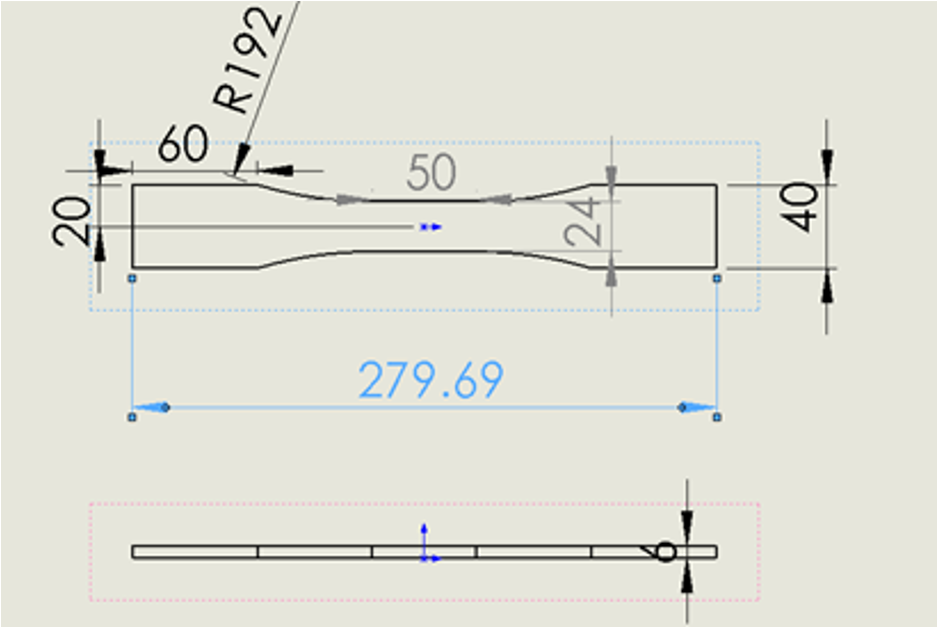
\includegraphics[height=0.7\textwidth]{fig/specimen_dim.png}
%     \caption{Schematic of the 5052-H32 aluminum alloy specimen}
%     \label{fig: specimen dim}
%   \end{subfigure}
%   \begin{subfigure}[t]{0.49\linewidth}
%     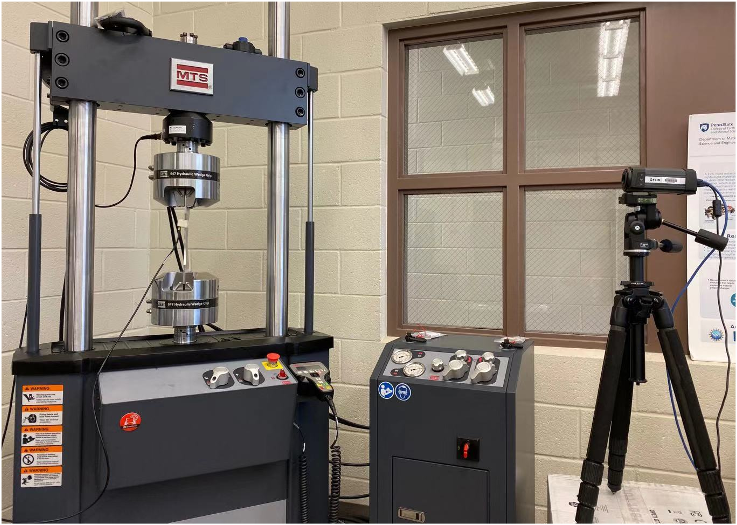
\includegraphics[height=0.7\textwidth]{fig/fatigue_testing_machine.png}
%     \caption{MTS 100KN Landmark fatigue testing system at Prof. Jingjing li's lab}
%     \label{fig: fatigue testing machine}
%   \end{subfigure}

%   \caption{Life cycle fatigue testing setup}
%   \label{fig: fatigue testing setup}
% \end{figure}

% \begin{figure}[tb]
%   \centering
%   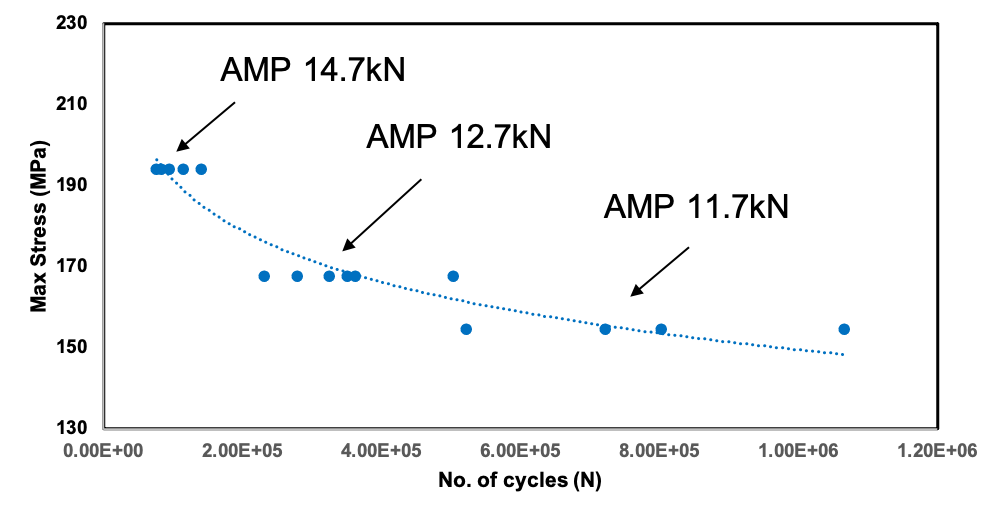
\includegraphics[width=0.8\linewidth]{fig/sn_curve.png}
%   \caption{S-N curve for 5052-H32 aluminum alloy}
%   \label{fig: raw sn curve}
% \end{figure}

\section{Interrupted fatigue testing}
The purpose of performing interrupted fatigue testing is to produce damaged specimens at various fatigue levels by stopping the testing at several predetermined numbers of cycles. Considering the material cost and the time spent, the number of cycles applied to the specimens is set to be two levels, 33\% and 67\% fatigue life corresponding to the three loading amplitudes, 11.7, 12.7, and 14.7 kN. These specimens are used to represent the end-of-life products at different fatigue damage levels from the remanufacturing industry. Besides, three specimens without going through fatigue testing, i.e., 0\% fatigue life, are included as specimens at the healthy state. The summary of the interrupted fatigue testing specimens is presented in Table \ref{table: interrupted specimens}

\begin{table}[tb]
  \centering
  \caption{Summary of the interrupted fatigue testing specimens}
  \label{table: interrupted specimens}
  \begin{tabularx}{0.9\textwidth}{
    >{\centering\arraybackslash}X
    >{\centering\arraybackslash}X
    >{\centering\arraybackslash}X
    >{\centering\arraybackslash}X
  }
    \toprule
    Specimen ID&Loading Amplitude (kN)&Percentage of Fatigue Life (\%)&Max Stress Applied (MPa)\\
    \midrule
    1&11.7&33&176\\
    2&11.7&33&176\\
    3&11.7&67&176\\
    4&11.7&67&176\\
    5&12.7&33&195\\
    6&12.7&33&195\\
    7&12.7&67&195\\
    8&12.7&67&195\\
    9&14.7&33&221\\
    10&14.7&33&221\\
    11&14.7&67&221\\
    12&14.7&67&221\\
    13&--&0&--\\
    14&--&0&--\\
    15&--&0&--\\
    \bottomrule
  \end{tabularx}
\end{table}

\section{Linear and nonlinear ultrasound measurements}
In this research, the LU and NLU testings serve as the two main NDE methods for measuring the accumulated fatigue damage in the specimens. 
% The ultrasonic testing is led by Prof. Matlack's group, and the testing system is shown in Figure \ref{fig: ultrasound setup}. 
The LU and NLU measurements are both 1-D time-domain signals, but the two approaches differ based on different theories and parameters, e.g., excitation wave shape, frequency, and amplitude. Examples of LU and NLU signals are presented in Figure \ref{fig: lu and nlu signals raw}.

LU and NLU measurements were collected at nine locations on a specimen as illustrated in Figure \ref{fig: measurement locations}, and each location was measured three times to ensure the measurement repeatability. As a result, for each specimen, there are $9 \times 3 = 27$ signal profiles produced. In total, the dataset contains 405 signal profiles.

% \begin{figure}[tb]
%   \centering
%   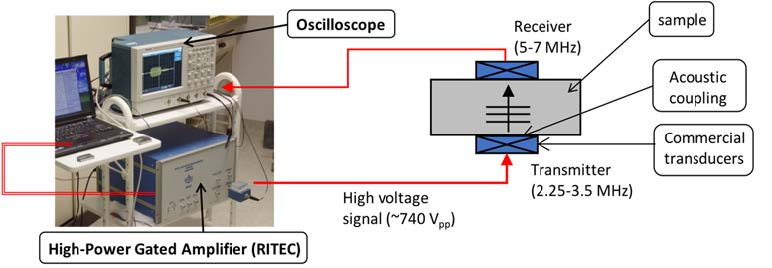
\includegraphics[width=0.9\linewidth]{fig/ultrasound setup.png}
%   \caption{Experimental setup for LU and NLU measurements at Prof. Matlack's Lab}
%   \label{fig: ultrasound setup}
% \end{figure}

\begin{figure}[tb]
  \centering
  \begin{subfigure}[t]{0.49\linewidth}
    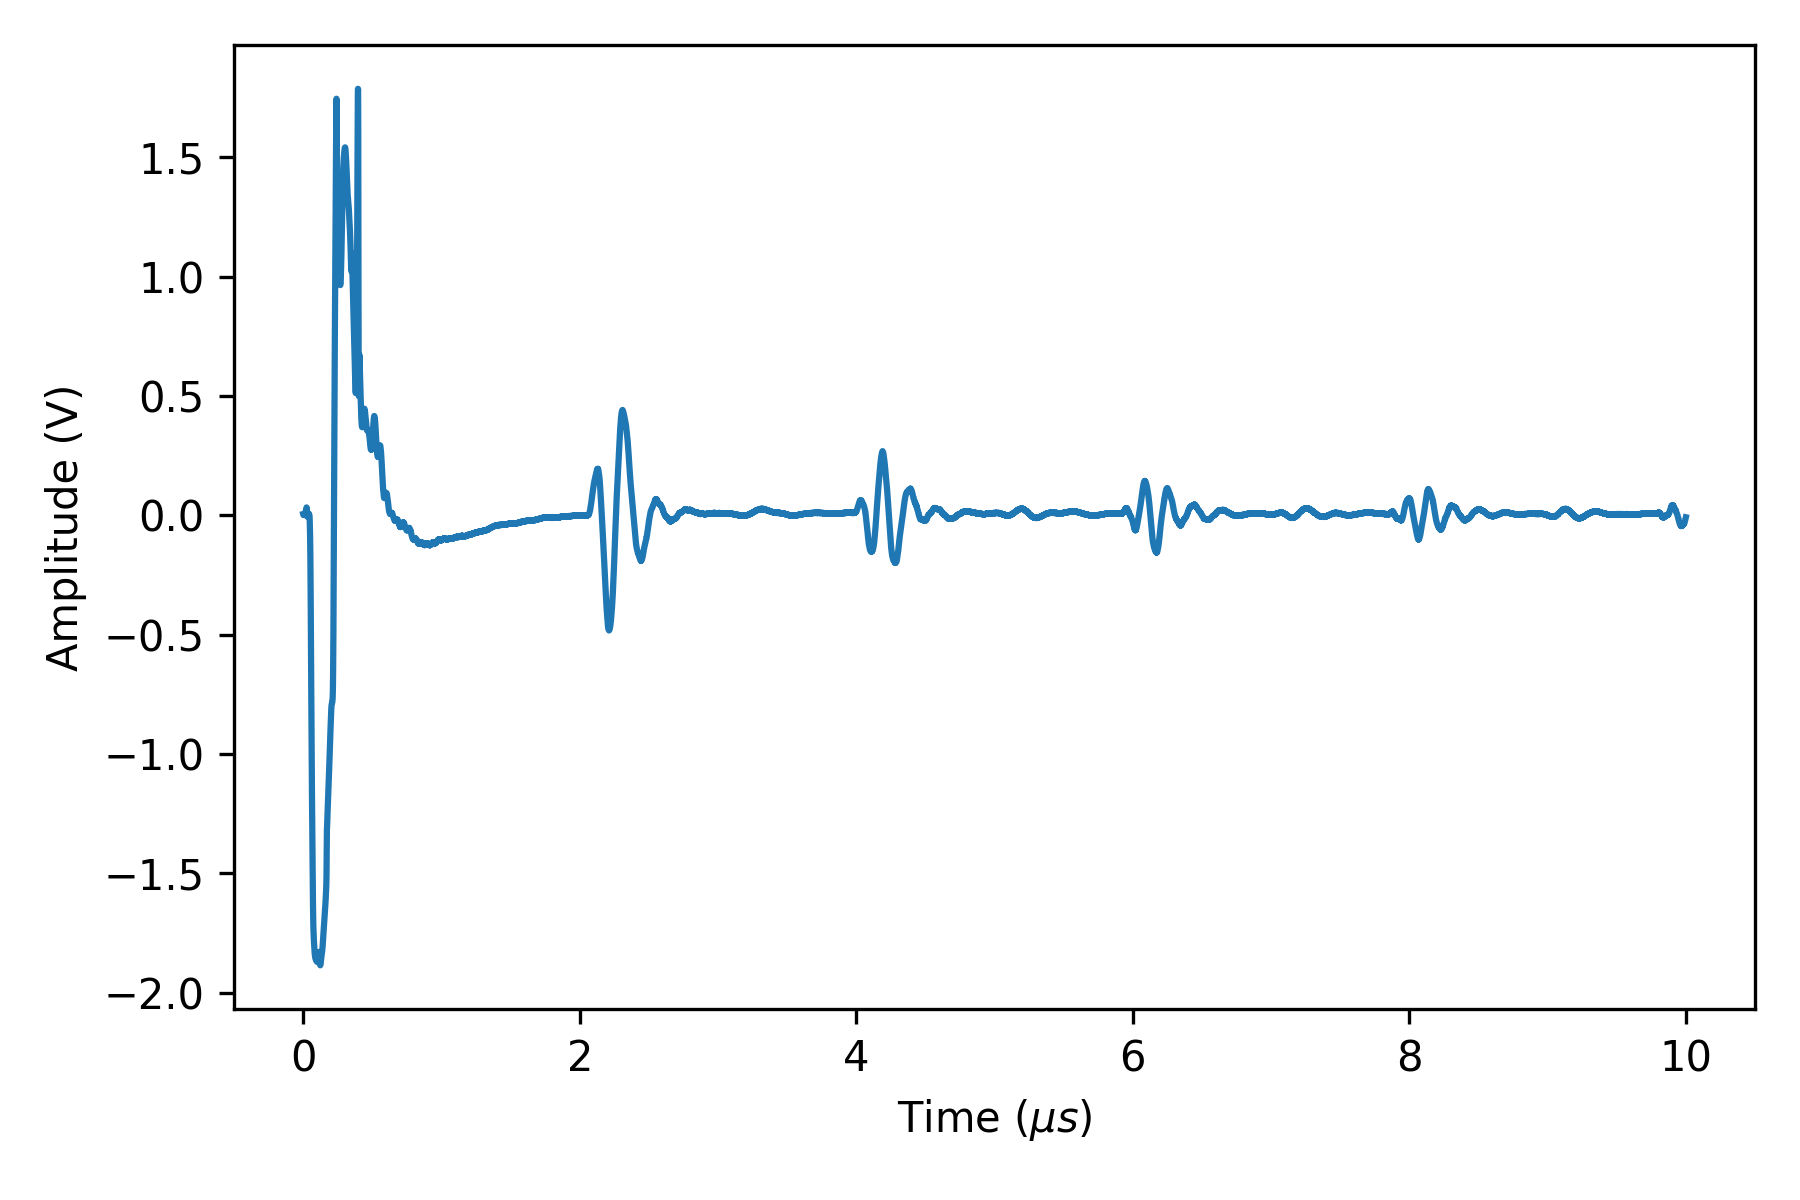
\includegraphics[width=\textwidth]{fig/lu_signal_raw.png}
    \caption{Linear ultrasonic signal}
    \label{fig: lu signal raw}
  \end{subfigure}
  \begin{subfigure}[t]{0.49\linewidth}
    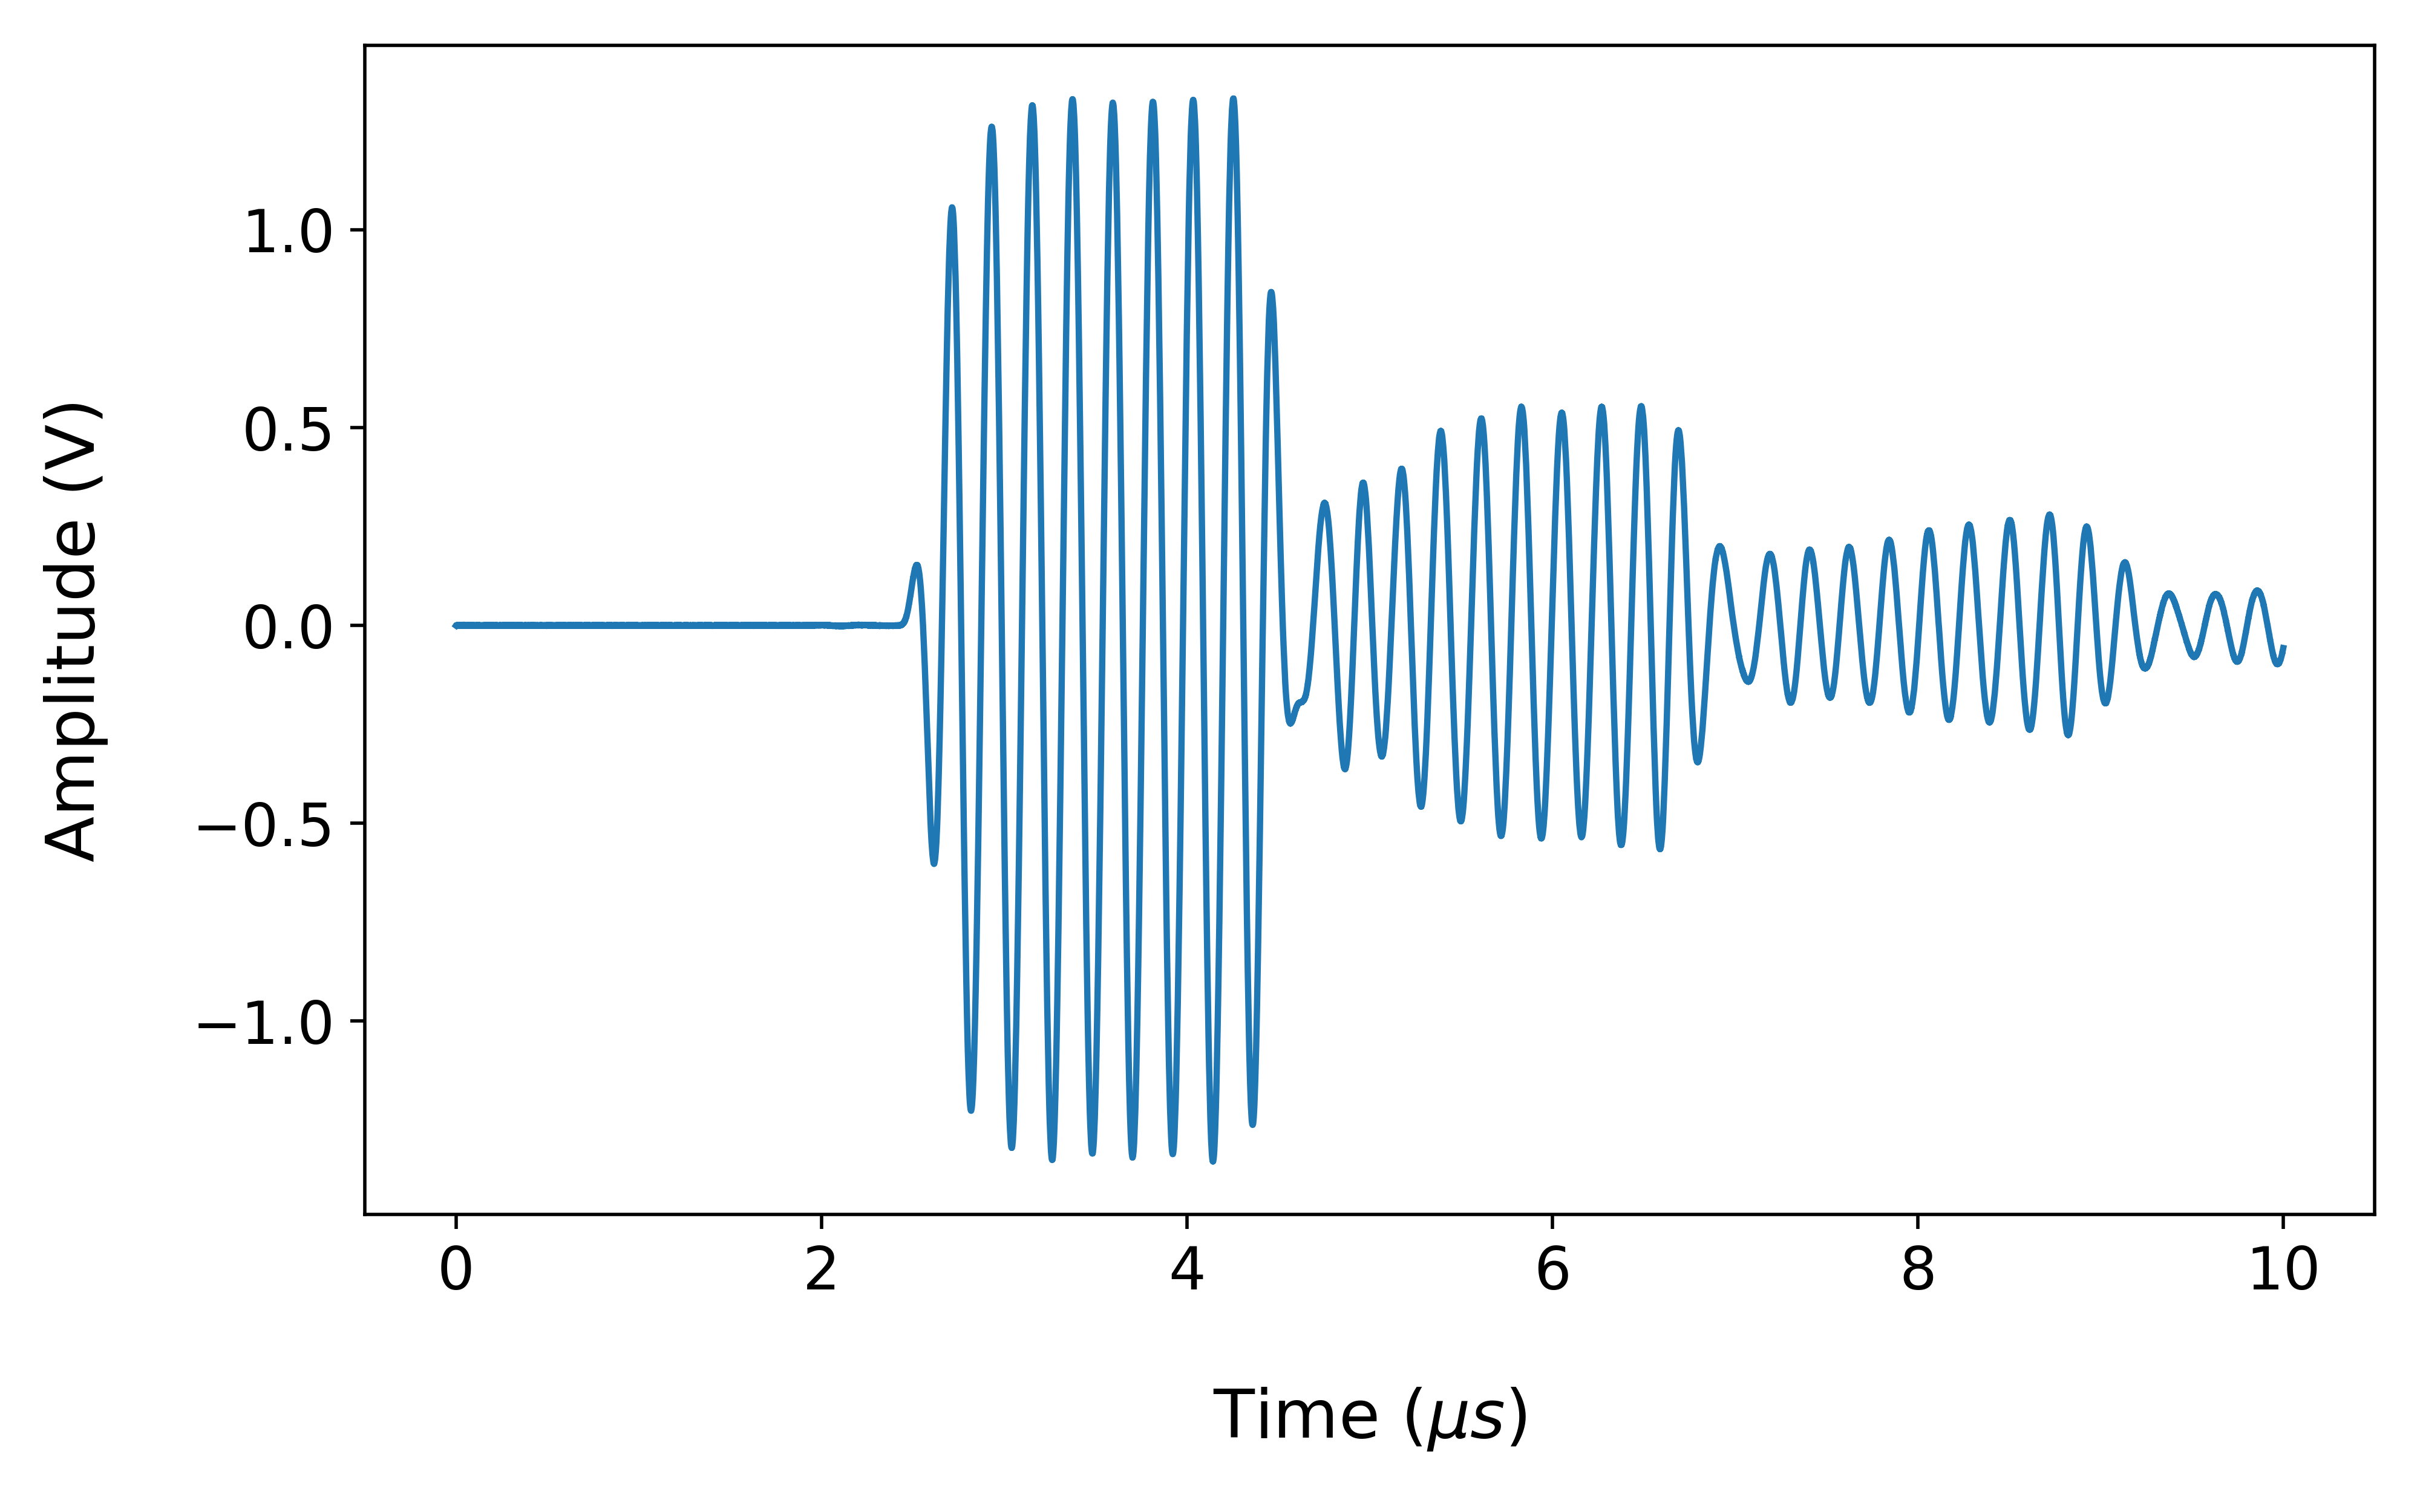
\includegraphics[width=\textwidth]{fig/nlu_singal_raw.png}
    \caption{Nonlinear ultrasonic signal}
    \label{fig: nlu signal raw}
  \end{subfigure}

  \caption{Examples of linear and nonlinear ultrasonic signals}
  \label{fig: lu and nlu signals raw}
\end{figure}

\begin{figure}[tb]
  \centering
  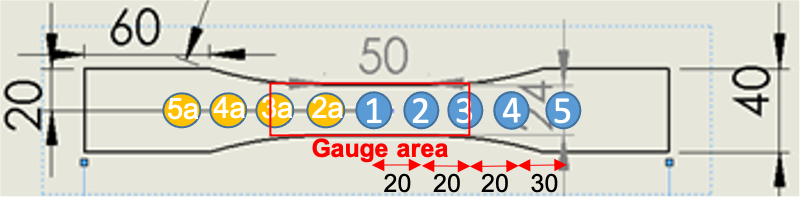
\includegraphics[width=0.6\linewidth]{fig/specimen_measurment_locs.png}
  \caption{Schematic of the measurement locations for LU and NLU measurements. (The unit is in mm)}
  \label{fig: measurement locations}
\end{figure}

\section{X-ray diffraction measurement}
Another quantity of interest, residual stress, is measured by XRD in this research. Residual stress is known to be associated with fatigue behaviors such as crack initiation and propagation. Besides, the FWHM height of the diffraction peak in XRD is also extracted. Prof. Li's group performed the XRD measurements for a subset of the specimens in the interrupted fatigue testing dataset. The residual stress and FWHM measured by XRD are used in the regression tasks in Chapter \ref{chap: reg} as target variables.
 % for EXPERIMENTS in "exper.tex"
\chapter{Model Development}
\label{chap: model}

This chapter introduces a model development procedure used in both classification tasks in Chapter \ref{chap: rul} and regression tasks in Chapter \ref{chap: reg}. The procedure involves:
\begin{enumerate*}[label=\itshape\alph*\upshape)]
    \item signal pre-processing,
    \item feature generation,
    \item feature selection,
    \item model training,
    \item model validation, and
    \item hyperparameter tuning,
\end{enumerate*}
as shown in Figure .

\section{Signal pre-processing}
It is essential to reduce noises and extract regions of interest from signals by signal processing before we perform other analyses. Figure presents this process. First, DC bias was removed by subtracting the mean amplitude of a signal to prevent models from fitting on bias. Second, Considering the computational cost from the high resolution data, we choose to downsample the ultrasonic signals. Third, we define the region or interest as the interval containing the ultrasonic signal responses, and the other parts of a signal are discarded so that redundant information is not included.

\section{Feature generation}
Since ultrasonic sensor signals are unstructured, which is difficult to process, feature extraction methods are needed to create a representative set of values, i.e., features that aggregate the information from an entire signal. In this stage, physics-based and data-driven features are generated. The hybrid feature pool enables us to incorporate physics knowledge into models.

\subsection{Physics-based features}
Given that physics modeling is built on theories or comprehensive experiment studies, physics-based features are robust, explainable, and suitable for applications having limited amounts of data. Therefore, features from traditional LU and NLU testings become potential candidates for the model.
\begin{itemize}
    \item Wave velocity
    
    In LU testing, ultrasonic wave velocity is a stiffness based measure which is associated with macroscopic damage such as crack/void coalescence and propagation. The wave speed is the distance divided by the time-of-flight (TOF) that a ultrasonic wave transverses in the material, as shown by Equation \eqref{eq: wave velocity}
    
    \begin{equation}
        v = \frac{2D}{\Delta t}
        \label{eq: wave velocity}
    \end{equation}
    where wave velocity is denoted by $v$, and $D$ is the thickness of the specimen. $\Delta t$ is the time difference between the actuation pulse and the response signal. Notice that, in our LU testing setup, one transducer severs as both the transmitter and receiver. Thus, the excitation signal travels $2D$ and the phase is changed $180^{\circ} $ when received.

    \item Nonlinear acoustic parameter $\beta$
    
    While wave velocity from LU is able to detect fatigue damage at macro-scale, it is limited because it cannot detect defects much smaller than the probing wavelength, e.g., 1mm. In contrast, NLU techniques are based on a different physical principle: nonlinear elasticity from nano- and micro-scale defects induce harmonic generation. The nonlinear acoustic parameter is related to the amplitude of generated harmonics. This nonlinear parameter changes due to defects such as dislocations, local plastic strain, precipitates, and micro-cracks, all of which are orders of magnitude smaller than the probing wavelength. Here, we simply calculate the nonlinear parameter by using the ratio between the amplitude of the fundamental and the harmonic waves given by Equation \eqref{eq: beta}

    \begin{equation}
        \beta = \frac{A_2}{A_1}
        \label{eq: beta}
    \end{equation}
    where A1, A2 is the amplitude of the fundamental wave and the second-order harmonic wave, respectively.
\end{itemize}

\subsection{Data-driven features}

\section{Feature selection}
\section{Model training}
\section{Model validation}
\section{Hyperparameter tuning} % for MODELDEV in "model.tex"
\chapter{Remaining Useful Life Prediction}
\label{chap: rul}

In this chapter, we propose a framework for predicting RUL of EoL products based on the ultrasonic testing. The framework has two parts: \begin{enumerate*}[label=\itshape\alph*\upshape)]
    \item a ML classification task and
    \item a RUL inference procedure based on S-N curve.
\end{enumerate*}  First, a ultrasonic signal is fed into ML classifiers to predict the loading condition and the number of fatigue cycles that a sample has gone through. Second, we estimate RUL from S-N curve with the predicted loading condition and fatigue cycles. % for RUL in "rul.tex"
\chapter{Residual Stress and FWHM Prediction}
\label{chap: reg}

Because of the efficiency of ultrasonic testings in terms of inspection area and cost, we explore the potential of using ultrasonic testings to measure quantities of interest, residual stress and full width at half maximum (FWHM), which are originally obtained from XRD analysis. In this chapter, we present regression models for predicting the residual stress and the FWHM of XRD peaks in fatigue damaged samples based on the ultrasonic measurements. 

\section{Problem formulation}
Following the same manner in Section \ref{sec: rul prob formulation}, we first translate the prediction tasks into ML regression problems based on the available dataset.

\subsection{Dataset}
The dataset for predicting residual stress and FWHM is composed of the XRD results and ultrasonic measurements. To obtain the residual stress and FWHM, the XRD analysis was performed on a subset of samples, containing 8 specimens and 3 measurement locations for each specimen, in the RUL dataset. Table \ref{table: rs dataset} and \ref{table: fwhm dataset} are the summary of the residual stress and FWHM dataset, respectively. It is observed that specimen 7's relatively low FWHM values could indicate that there are microcrack initiations, and the discussion about cracks in specimen 7 is presented in Section \ref{sec: reg discussion}.

\begin{table}[tb]
    \centering
    \caption{Summary of the residual stress prediction dataset}
    \label{table: rs dataset}
    \begin{tabularx}{\textwidth}{
      >{\centering\arraybackslash}X
      >{\centering\arraybackslash}X
      >{\centering\arraybackslash}X
      >{\centering\arraybackslash}X
    }
    \toprule
    Specimen ID & \multicolumn{3}{c}{Residual Stress (MPa)}\\
    \cmidrule(lr){2-4}
       & Location 1 & Location 2 & Location 3\\
      \midrule
      2 & -61.7 & -75.6 & -80.2 \\
      4 & -59.9 & -69.6 & -76.6 \\
      6 & -60.3 & -75.3 & -79.6 \\
      7 & -50.8 & -59.6 & -66.2 \\
      8 & -57.3 & -65.5 & -79.7 \\
      10 & -43.3 & -47.0 & -50.8 \\
      12 & -38.8 & -43.2 & -50.0 \\
      14 & -79 & -76.7 & -85.7 \\
      \bottomrule
    \end{tabularx}

    \footnotesize{The negative sign indicates the compressive residual stresses.}
\end{table}


\begin{table}[tb]
    \centering
    \caption{Summary of the FWHM prediction dataset}
    \label{table: fwhm dataset}
    \begin{tabularx}{\textwidth}{
      >{\centering\arraybackslash}X
      >{\centering\arraybackslash}X
      >{\centering\arraybackslash}X
      >{\centering\arraybackslash}X
    }
    \toprule
    Specimen ID & \multicolumn{3}{c}{FWHM ($^{\circ}$)}\\
    \cmidrule(lr){2-4}
       & Location 1 & Location 2 & Location 3\\
      \midrule
      2 & 0.354 & 0.353 & 0.355 \\
      4 & 0.350 & 0.354 & 0.353 \\
      6 & 0.358 & 0.359 & 0.363 \\
      7 & 0.307 & 0.320 & 0.321 \\
      8 & 0.357 & 0.355 & 0.358 \\
      10 & 0.356 & 0.358 & 0.360 \\
      12 & 0.354 & 0.353 & 0.355 \\
      14 & 0.338 & 0.340 & 0.346 \\
      \bottomrule

    \end{tabularx}
\end{table}

\subsection{Target variables}
Residual stress and FWHM are the target variables in this chapter. Residual stress is known to influence fatigue behaviors including crack initiation and propagation. FWHM is also an indicator for evaluating crack propagation. As a result, accurately predicting residual stress and FWHM based on ultrasonic measurements is beneficial to assist fatigue level estimation. Here, the problem is formulated as two regression tasks separately:
\begin{enumerate*}[label=(\alph*)]
    \item a univariate regression with residual stress as the target variable, and
    \item a univariate regression with FWHM as the target variable.
\end{enumerate*}


\section{Residual stress prediction}
\label{sec: rs prediction}
A regression model, RFECV-SVM\textsubscript{RS}, for predicting residual stress based on ultrasonic signals is developed by following the procedure in Chapter \ref{chap: model}. Besides, the RFECV-SVM\textsubscript{RS} model is compared with other approaches such as Lasso regression, linear regression with top 5 features from Lasso regression, and random forest. Root mean squared error (RMSE) and mean absolute percentage error (MAPE) are used to assess the model performance with LOGOCV results, as shown in Table \ref{table: summary rs model}. In this task, the RFECV-SVM\textsubscript{RS} model performs the best with the MAPE equal 4.73\%. Figure \ref{fig: rs prediction} illustrates the RFECV-SVM\textsubscript{RS} model prediction by showing the actual and predicted residual stresses, in which a perfect model should follow the black line. It is observed that in most groups, at least one prediction among three repeated measurements (three predictions for the same actual residual stress in one sample group) is close to the ideal prediction, and the MAPEs for each group are mostly below 10\%.

\begin{table}[tb]
    \centering
    \caption{Summary of regression models for residual stress estimation and model performance}
    \label{table: summary rs model}
    \begin{tabularx}{\textwidth}{
      >{\centering\arraybackslash}X
      >{\centering\arraybackslash}X
      >{\centering\arraybackslash\hsize=0.8\hsize}X
      >{\centering\arraybackslash\hsize=0.8\hsize}X
    }
    \toprule
    \multirow{2}{*}{Method}  & \multirow{2}{*}{\parbox{\linewidth}{\centering No. Selected \\ Features}} & \multicolumn{2}{c}{LOGOCV Test} \\
    \cmidrule(lr){3-4}
    & & RMSE (MPa) & MAPE (\%) \\
    \midrule
    %
    Lasso regression & 37 & 5.90 & 8.71 \\
    Linear regression & 5 & 4.92 & 7.54 \\
    Random forest & 191 & 7.74 & 12.85 \\
    \textbf{RFECV-SVM} & 29 & \textbf{3.24} & \textbf{4.73} \\
    \bottomrule
    \end{tabularx}
\end{table}

\begin{figure}[tb]
  \centering
  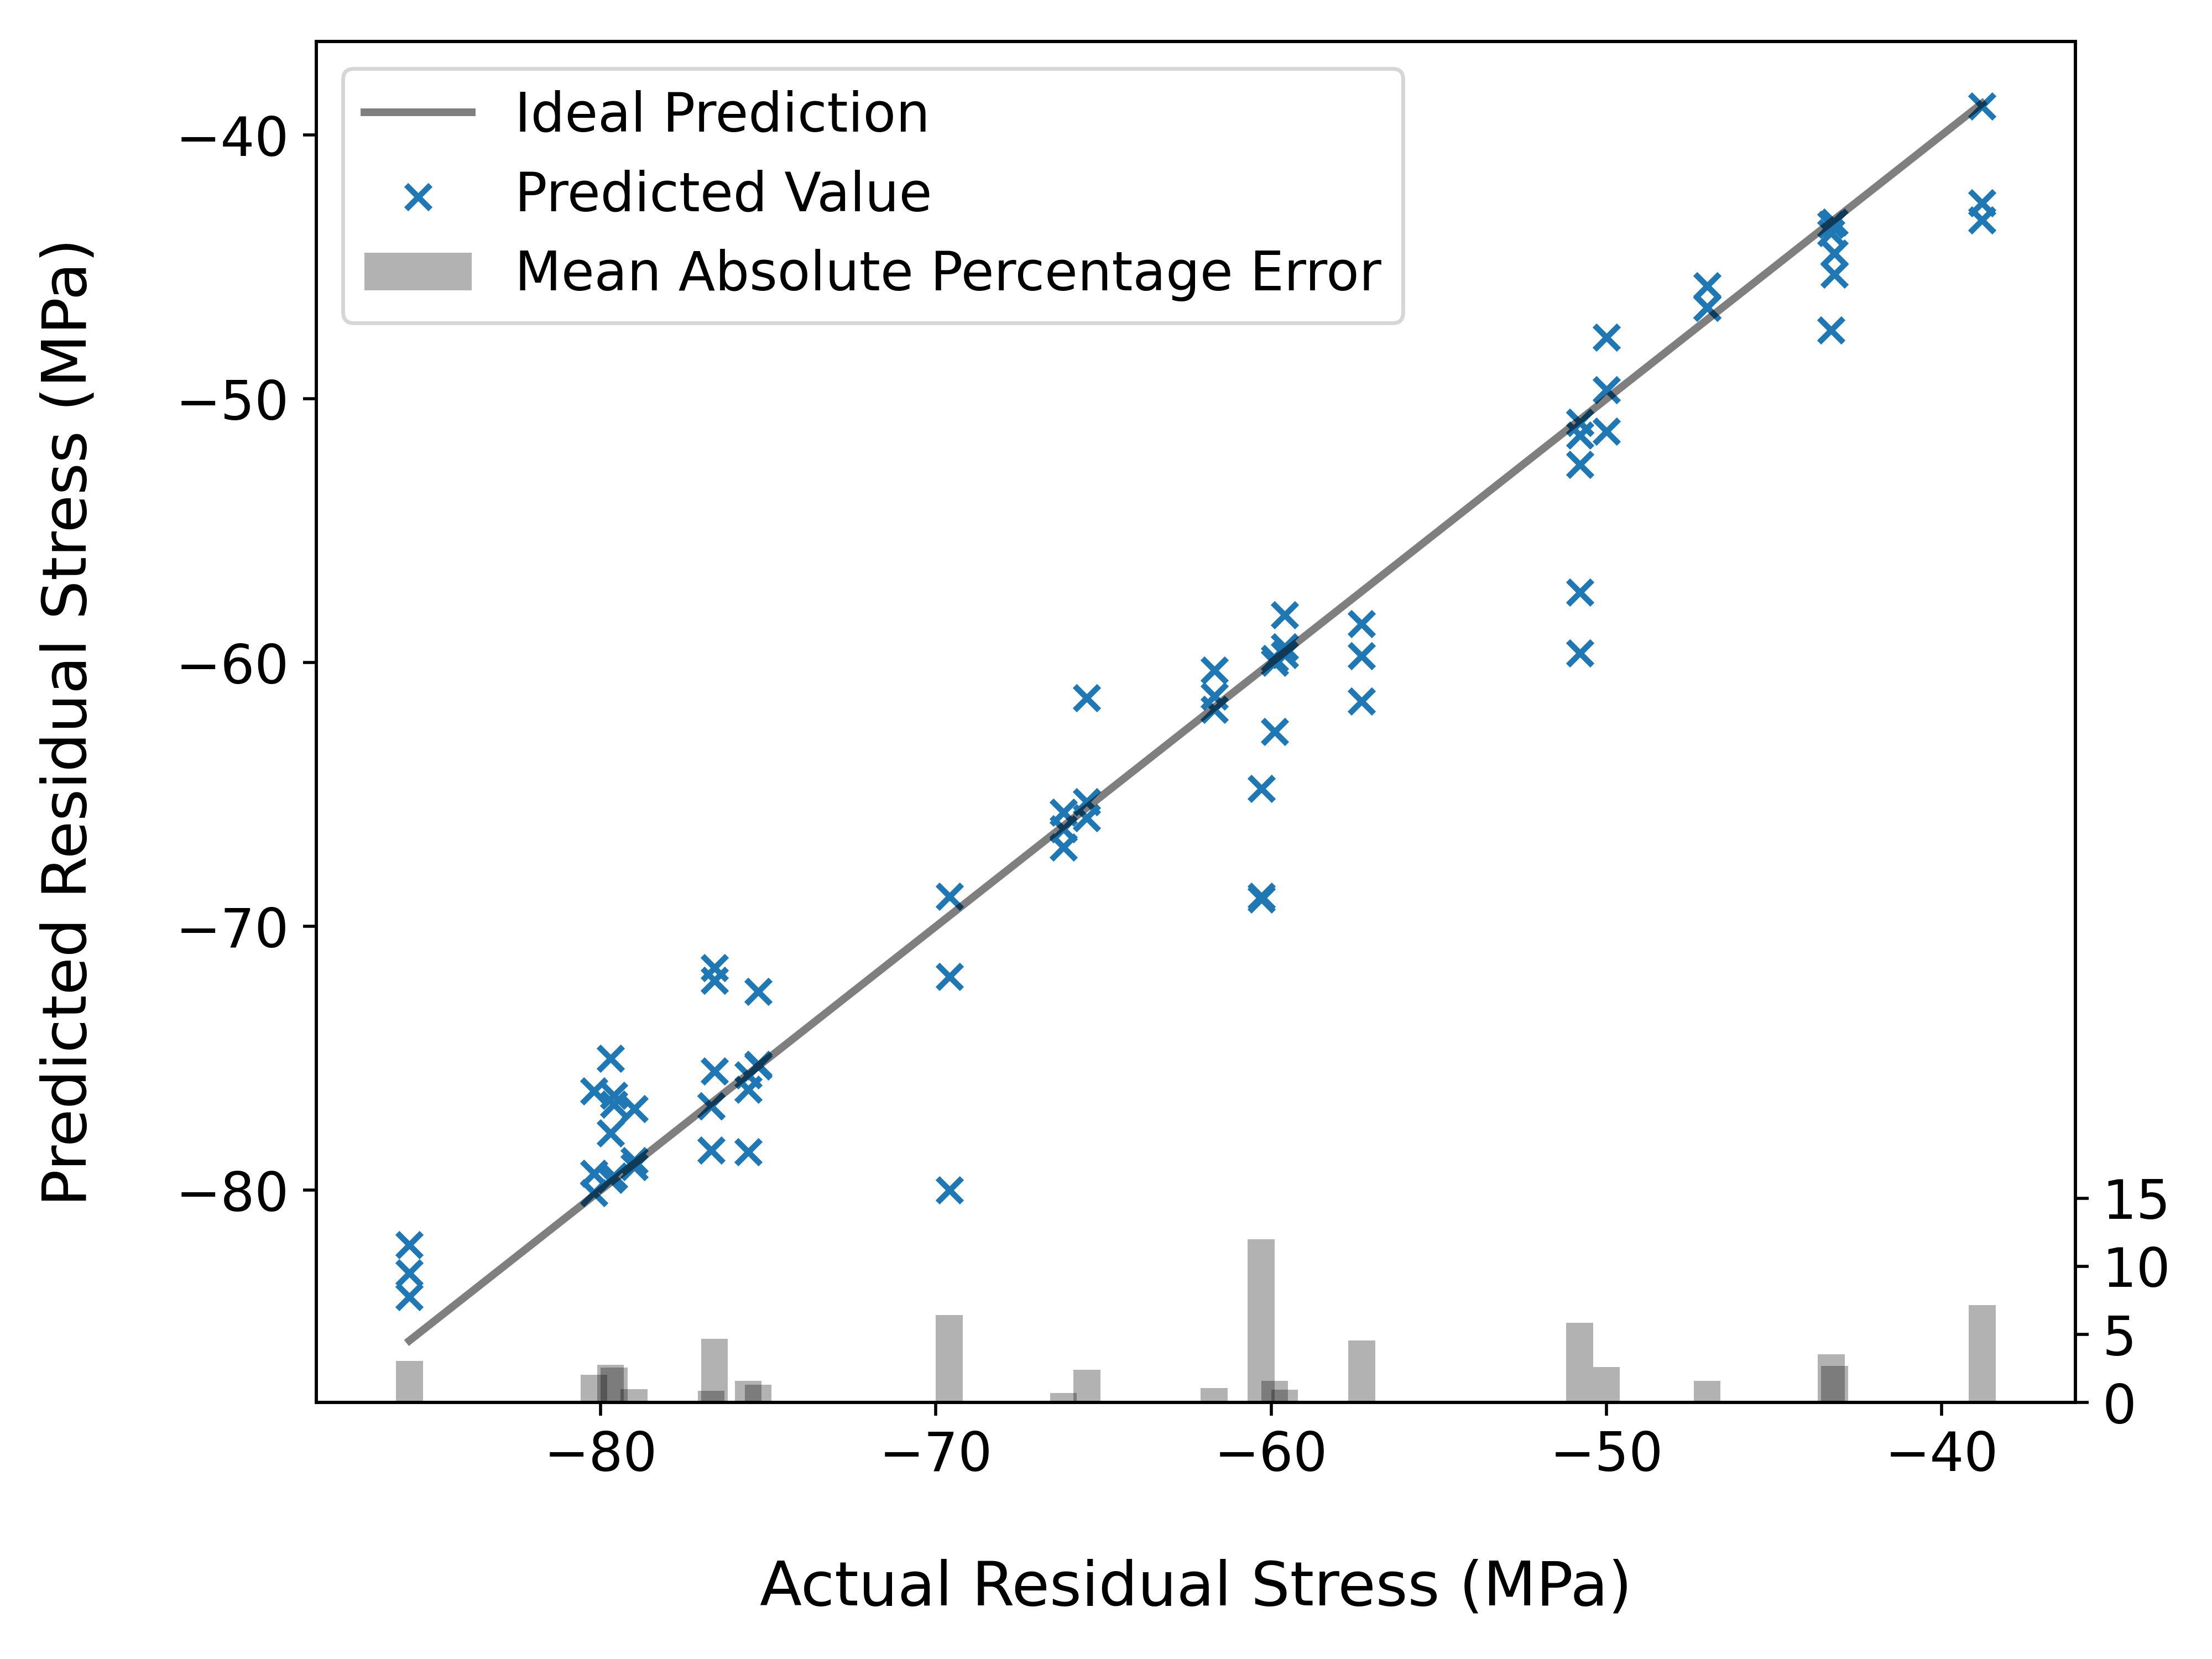
\includegraphics[width=0.8\linewidth]{fig/residual_stress_predict_vs_true.png}
  \caption{Scatter plot of actual vs predicted residual stress by RFECV-SVM}
  \label{fig: rs prediction}
\end{figure}

\section{FWHM prediction}
Similarly, an FWHM prediction model, RFECV-SVM\textsubscript{FWHM}, is built based on the procedure in Chapter \ref{chap: model} and is evaluated with the same metrics in Section \ref{sec: rs prediction}. Table \ref{table: summary fwhm model} is the comparison of the RFECV-SVM\textsubscript{FWHM} with other regression methods. It is worth mentioning that the linear regression model with the top 5 features selected from Lasso regression achieves a 1.89\% MAPE, performing slightly better than the RFECV-SVM\textsubscript{FWHM}. Figure \ref{fig: fwhm prediction lr} and \ref{fig: fwhm prediction svm} illustrate the predictions of the linear regression model and the RFECV-SVM\textsubscript{FWHM}, respectively. For the RFECV-SVM\textsubscript{FWHM}, one can observe that the predictions of the small FWHM values from specimen 7 significantly deviate from the ideal predictions; nevertheless, the linear regression model is able to make close predictions. As mentioned earlier, we surmise that specimen 7 had developed cracks and the difference in the model performance led us to have a further investigation about specimen 7 in Section \ref{sec: reg discussion}. Before performing further analysis, by excluding specimen 7, we can conclude that both models achieve a good performance in predicting FWHM with errors less than 2\%.

\begin{table}[tb]
  \centering
  \caption{Summary of regression models for FWHM prediction and model performance}
  \label{table: summary fwhm model}
  \begin{tabularx}{\textwidth}{
    >{\centering\arraybackslash\hsize=1.2\hsize}X
    >{\centering\arraybackslash}X
    >{\centering\arraybackslash\hsize=0.75\hsize}X
    >{\centering\arraybackslash\hsize=0.75\hsize}X
  }
  \toprule
  \multirow{2}{*}{Method}  & \multirow{2}{*}{\parbox{\linewidth}{\centering No. Selected \\ Features}} & \multicolumn{2}{c}{LOGOCV Test} \\
  \cmidrule(lr){3-4}
  & & RMSE ($^{\circ}$) & MAPE (\%) \\
  \midrule
  %
  Lasso regression & 20 & 0.0081 & 2.40 \\
  \textbf{Linear regression} & 5 & \textbf{0.0056} & \textbf{1.62} \\
  Random forest & 191 & 0.0099 & 2.81 \\
  \textbf{RFECV-SVM} & 7 & \textbf{0.0063} & \textbf{1.89} \\
  \bottomrule
  \end{tabularx}
\end{table}

\begin{figure}[tb]
  \centering
  \begin{subfigure}[t]{\linewidth}
    \centering
    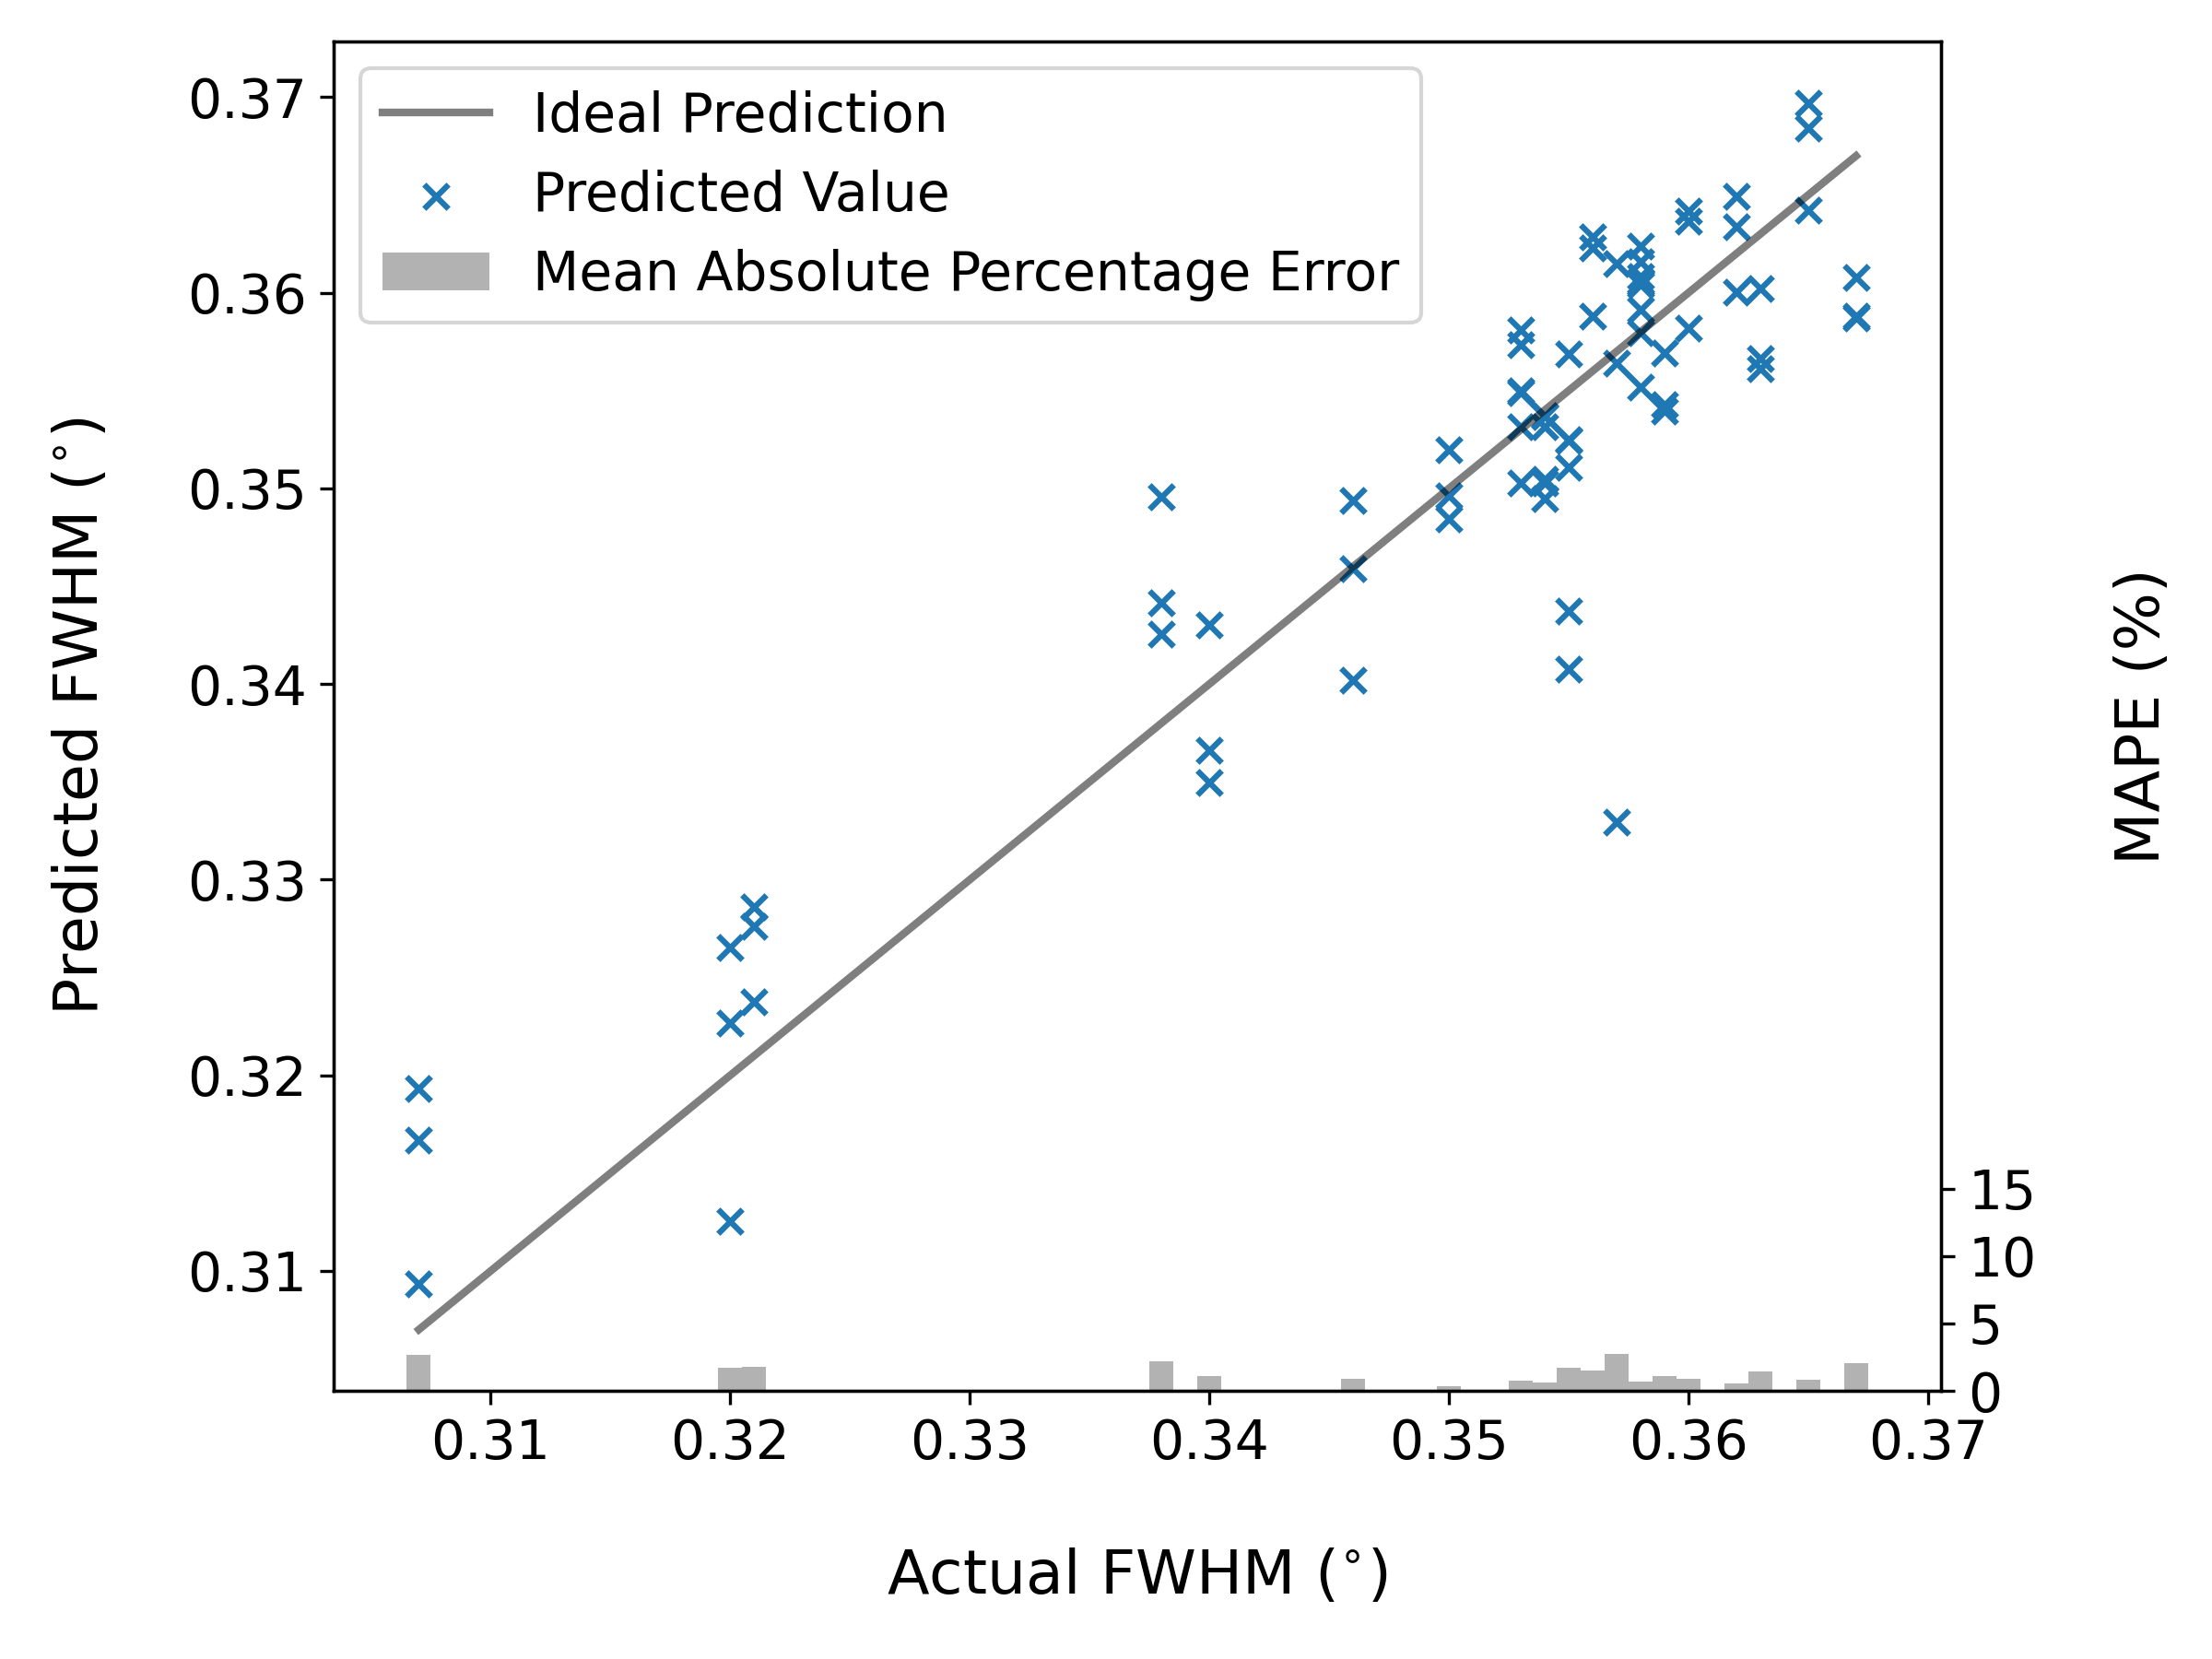
\includegraphics[width=0.8\linewidth]{fig/fwhm_predict_vs_true_lr.png}
    \caption{Linear regression}
    \label{fig: fwhm prediction lr}
  \end{subfigure}
  \begin{subfigure}[t]{\linewidth}
    \centering
    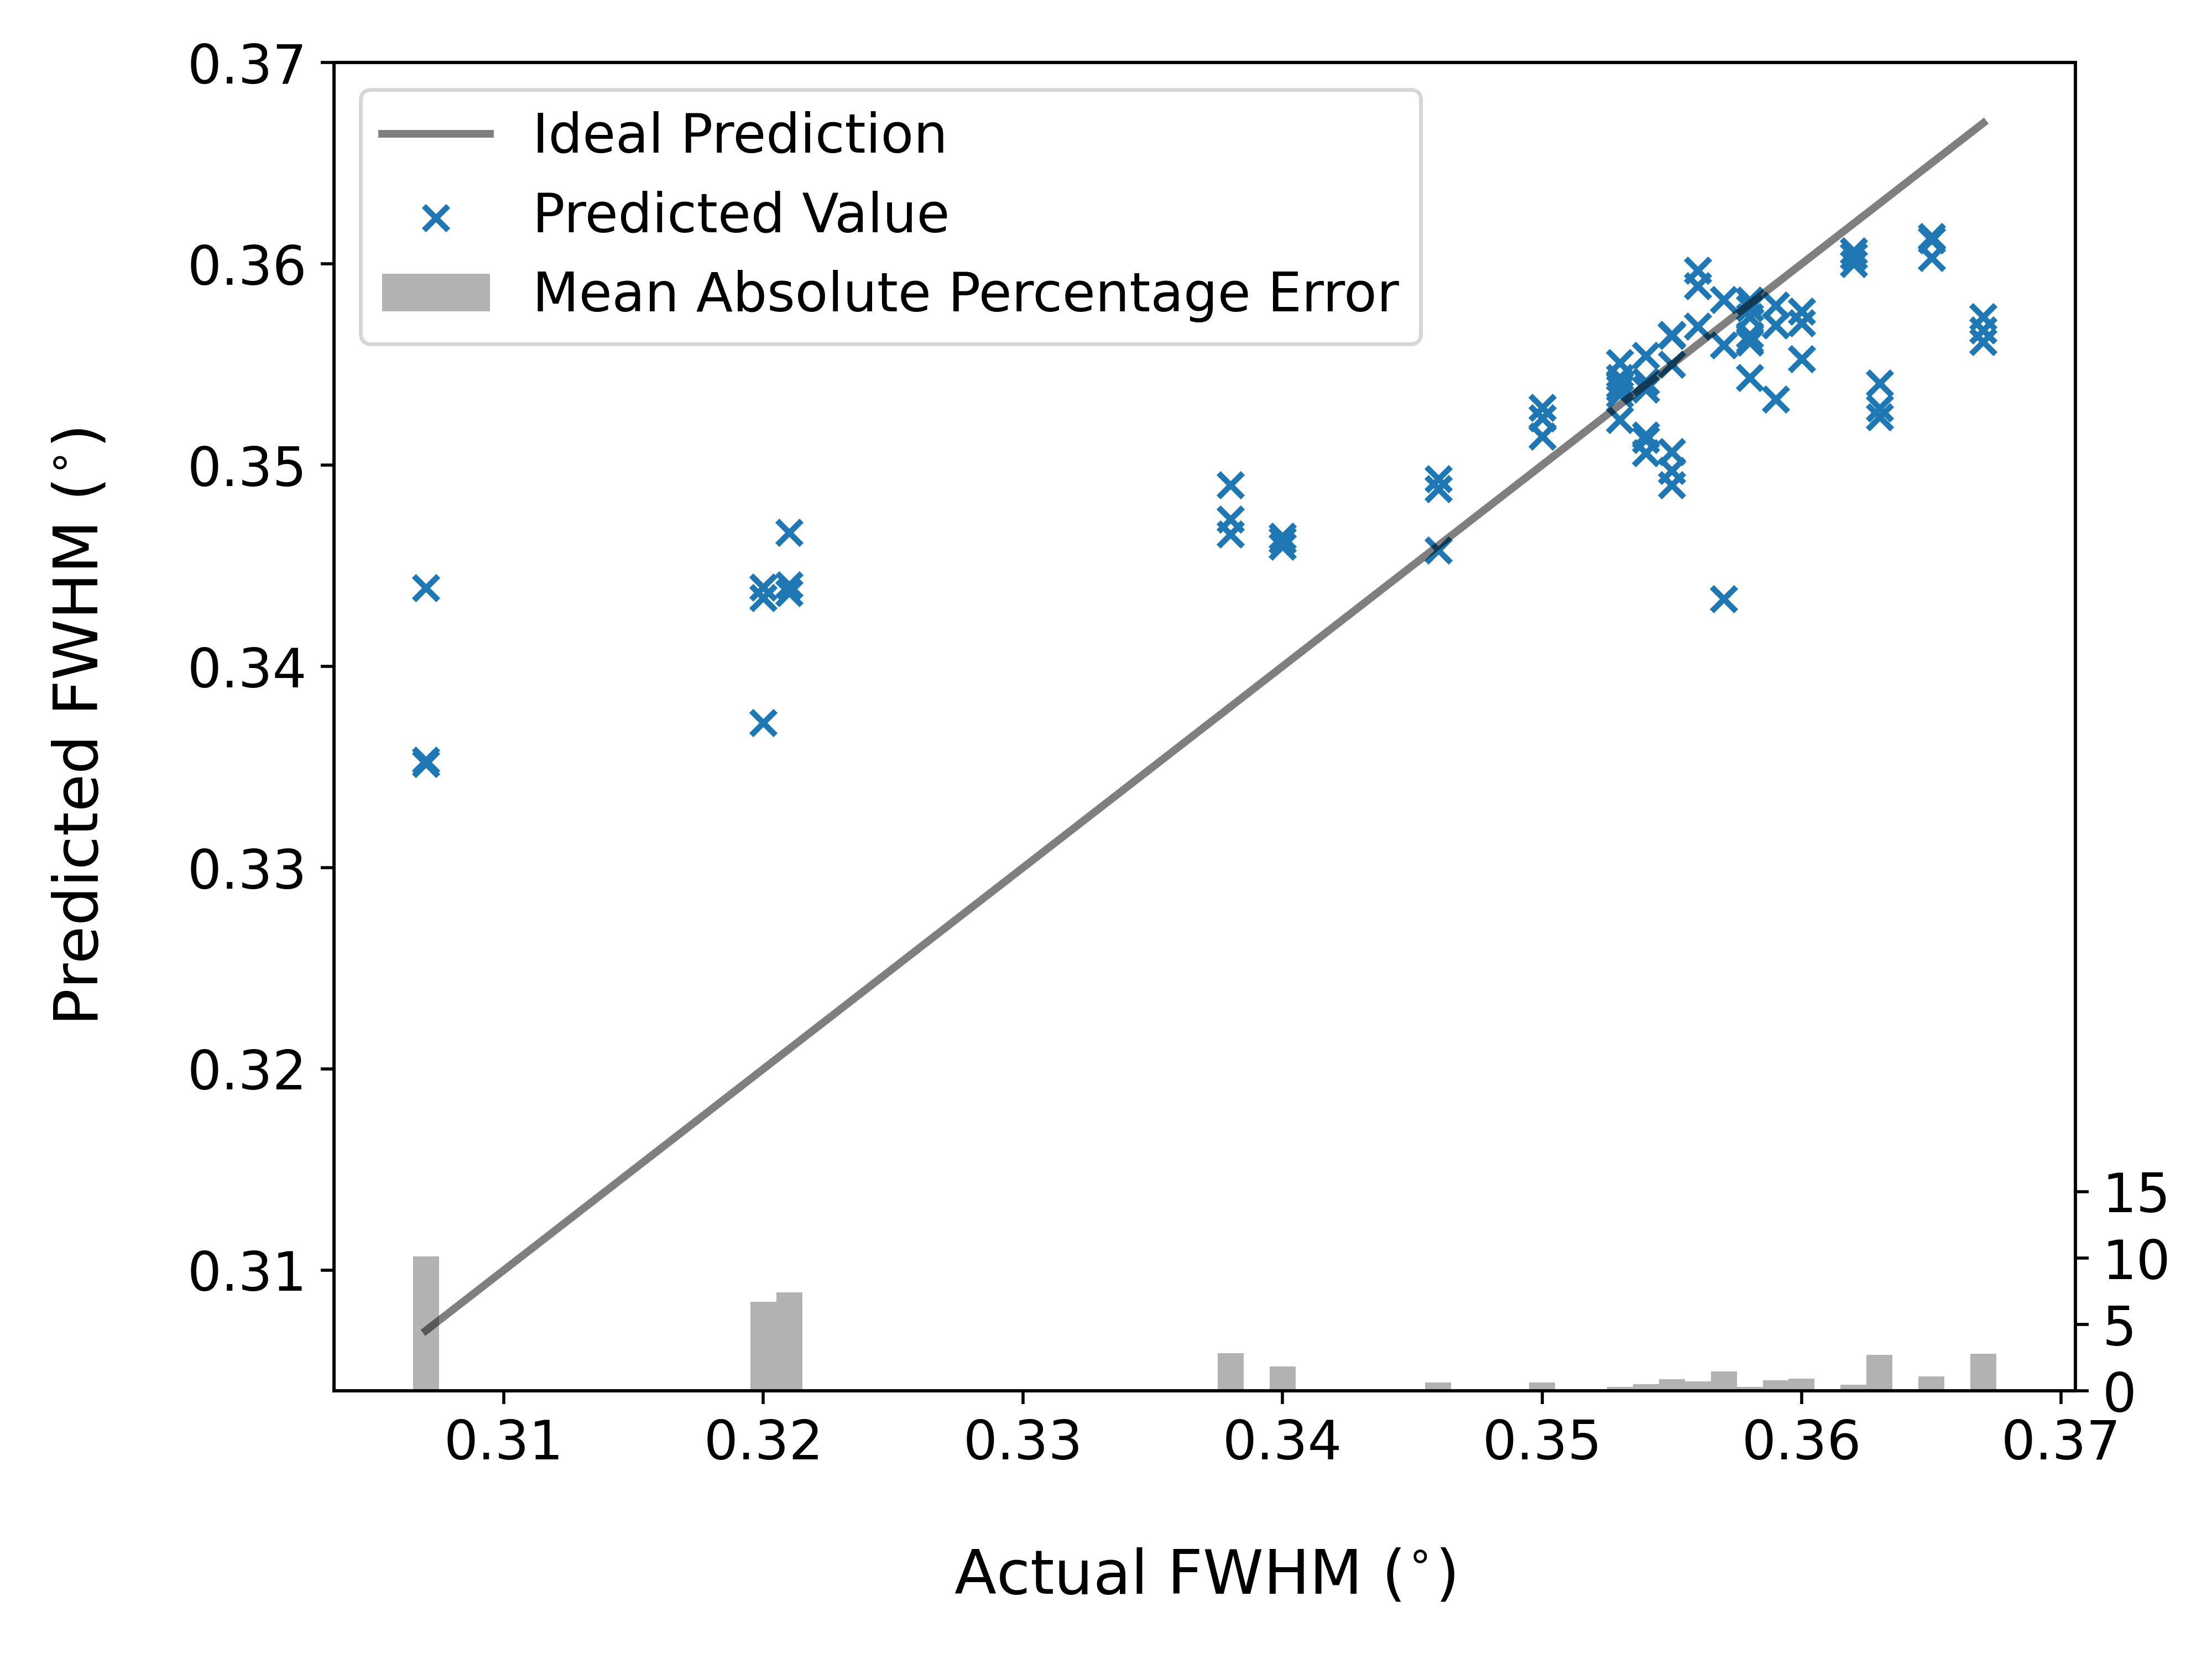
\includegraphics[width=0.8\linewidth]{fig/fwhm_predict_vs_true_svm.png}
    \caption{RFECV-SVM}
    \label{fig: fwhm prediction svm}
  \end{subfigure}

  \caption{Scatter plot of actual vs predicted FWHM}
  \label{fig: fwhm prediction}
\end{figure}

\section{Discussion}
\label{sec: reg discussion}
In this section, since we conjecture that specimen 7 had developed cracks based on the relatively small FWHM values measured from XRD analysis, the potential of using our ultrasonic technology to detect cracks is discussed.

\subsection{Crack detection through LU and NLU measurements}
To investigate whether our ultrasonic technology can detect cracks or not, we first assume specimen 7 is cracked and the differences in ultrasonic signals between specimen 7 and specimen 8 were resulted from the existence of cracks since specimen 7 and 8 were under the same experimental setting. Secondly, independent t-test is performed to test if the mean of a feature is significantly different between two groups, specimen 7 (15 measurements from location 3a to 3) and specimen 8 (15 measurements from location 3a to 3). Finally, Figure \ref{fig: crack detection feat dist} displays several specimen 7's and specimen 8's probability density plots of the selected features. The distributions are not identical between specimen 7 and 8, indicating that these features are possible to distinguish cracked samples from normal samples; however, given that we only have two specimens in this test and there exist other factors causing the differences in measurement signals, further research on crack detection through our ultrasonic technology is required.

\begin{figure}[tb]
  \begin{subfigure}[t]{0.49\linewidth}
    \centering
    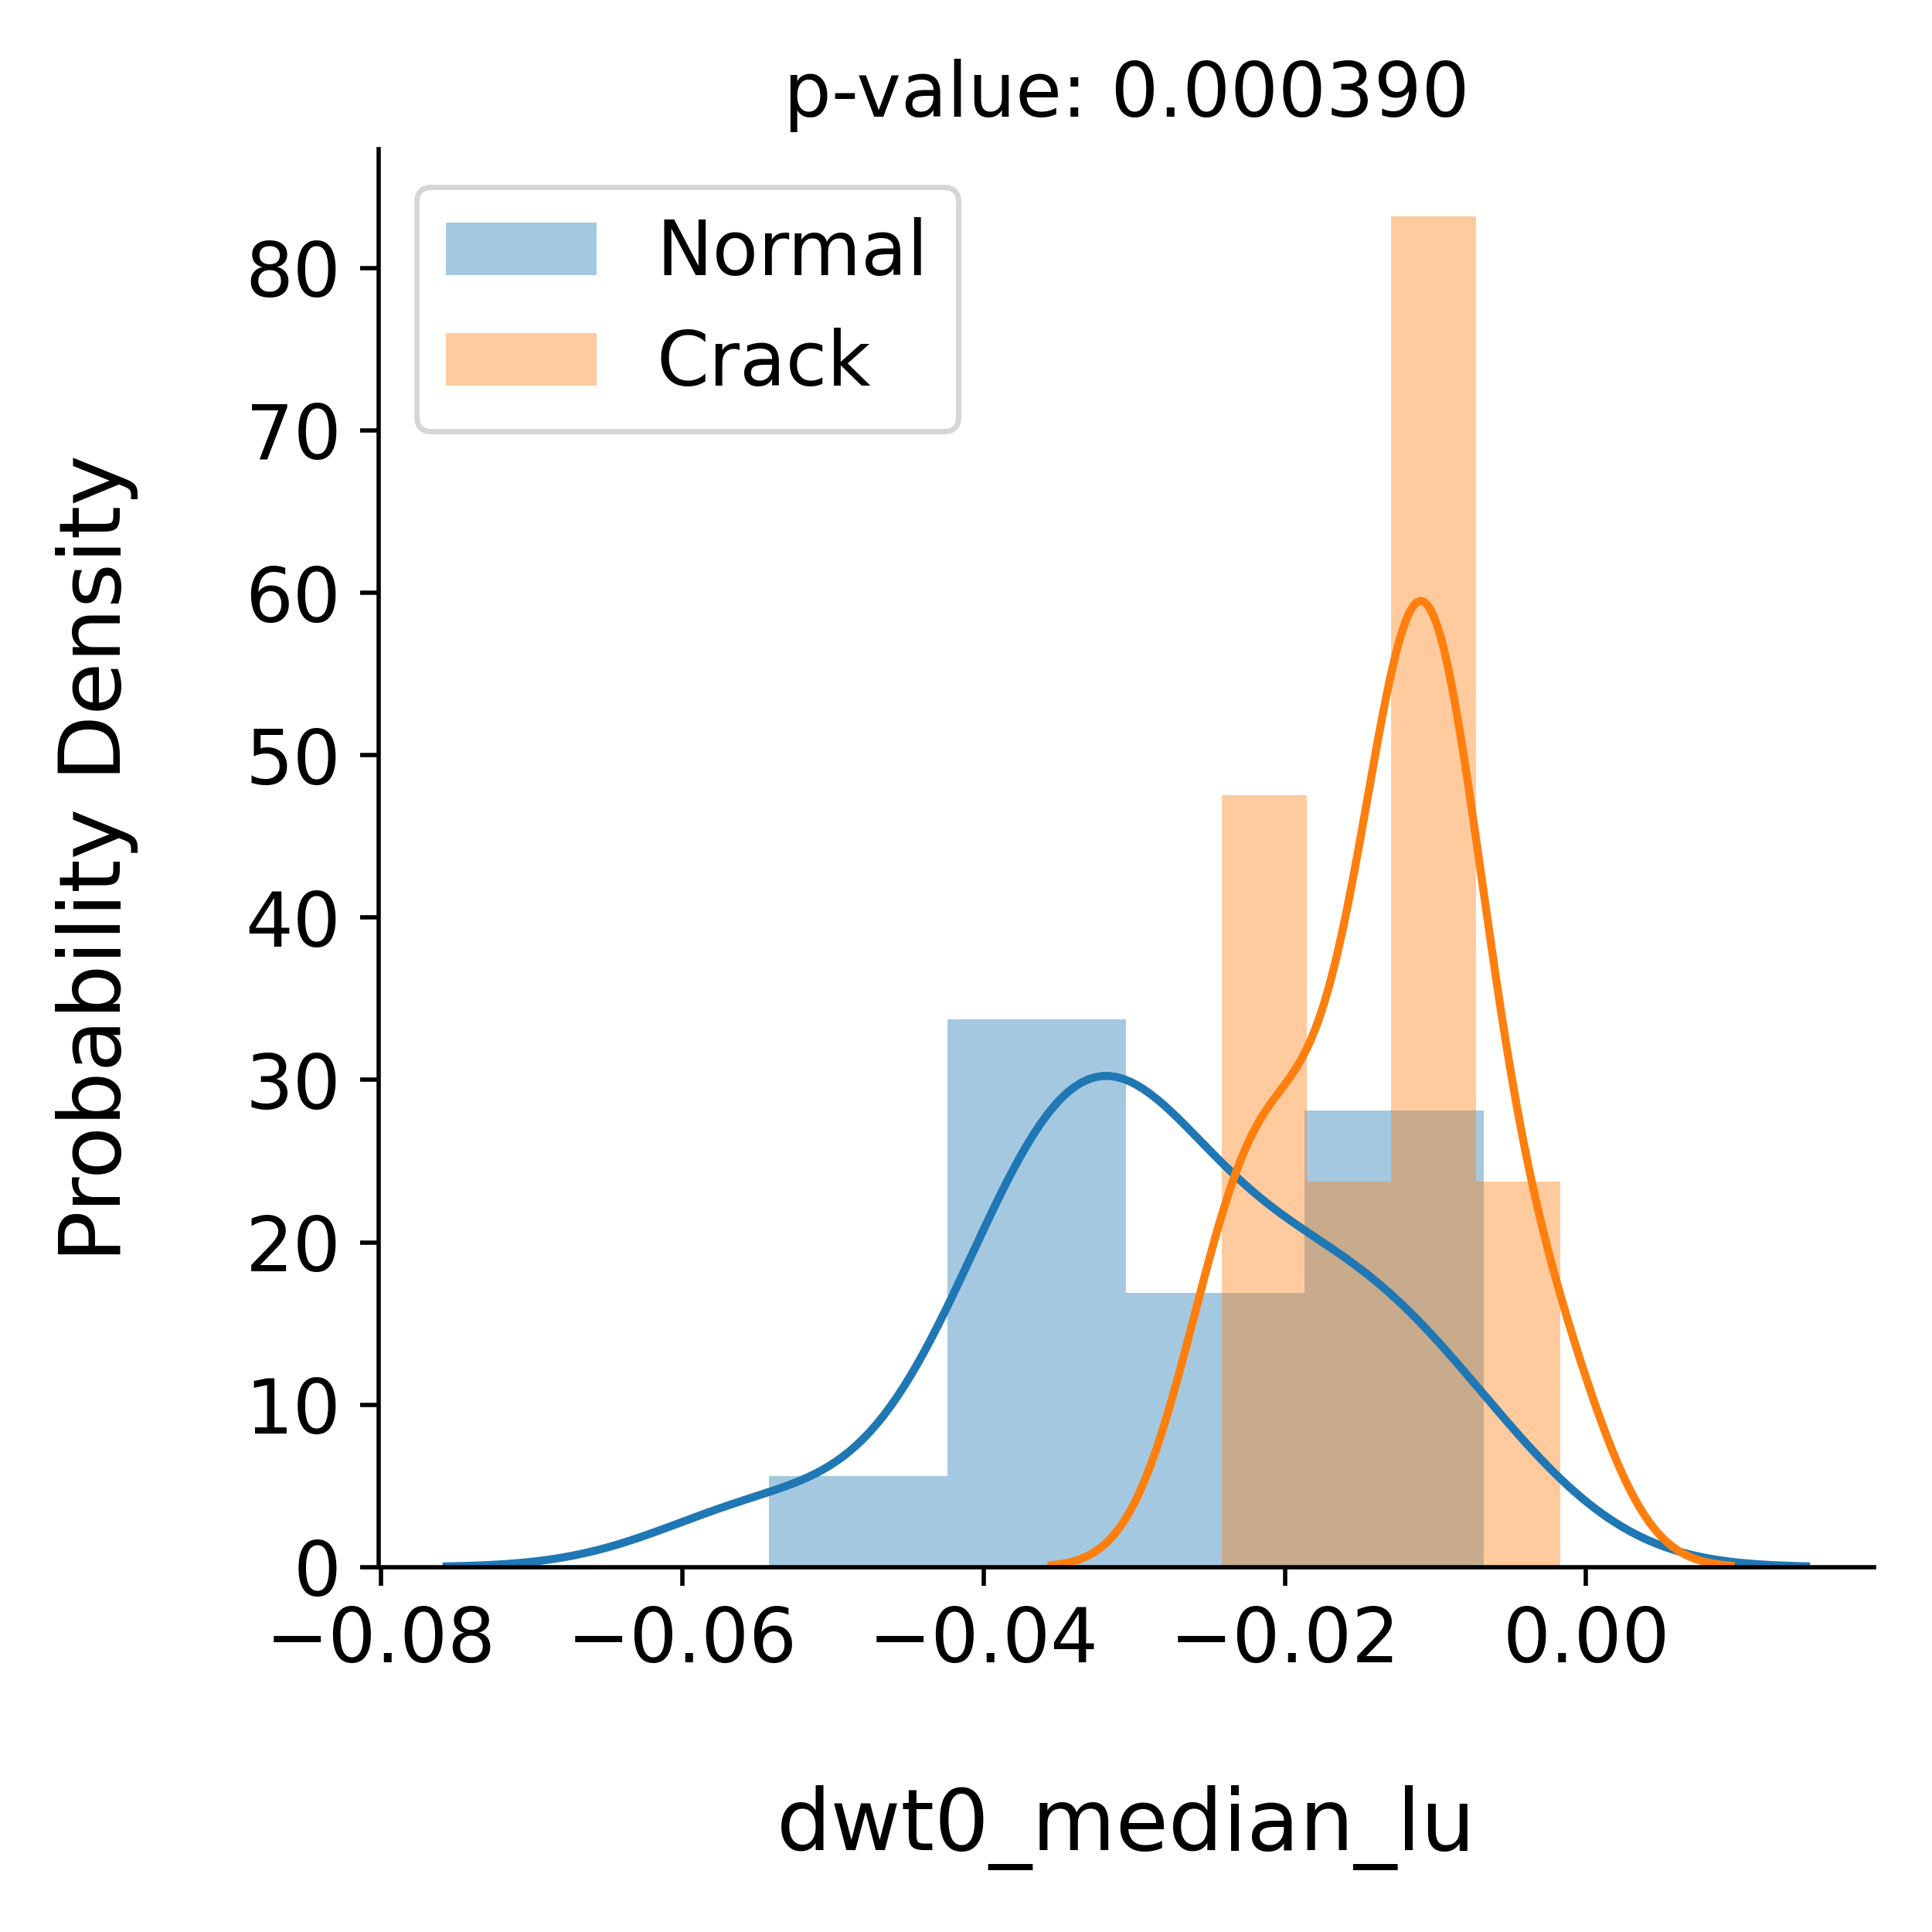
\includegraphics[width=0.8\textwidth]{fig/crack_detection_dwt0_median_lu.png}
    \caption{Median of level 0 DWT coefficient of LU signal}
  \end{subfigure}
  \begin{subfigure}[t]{0.49\linewidth}
    \centering
    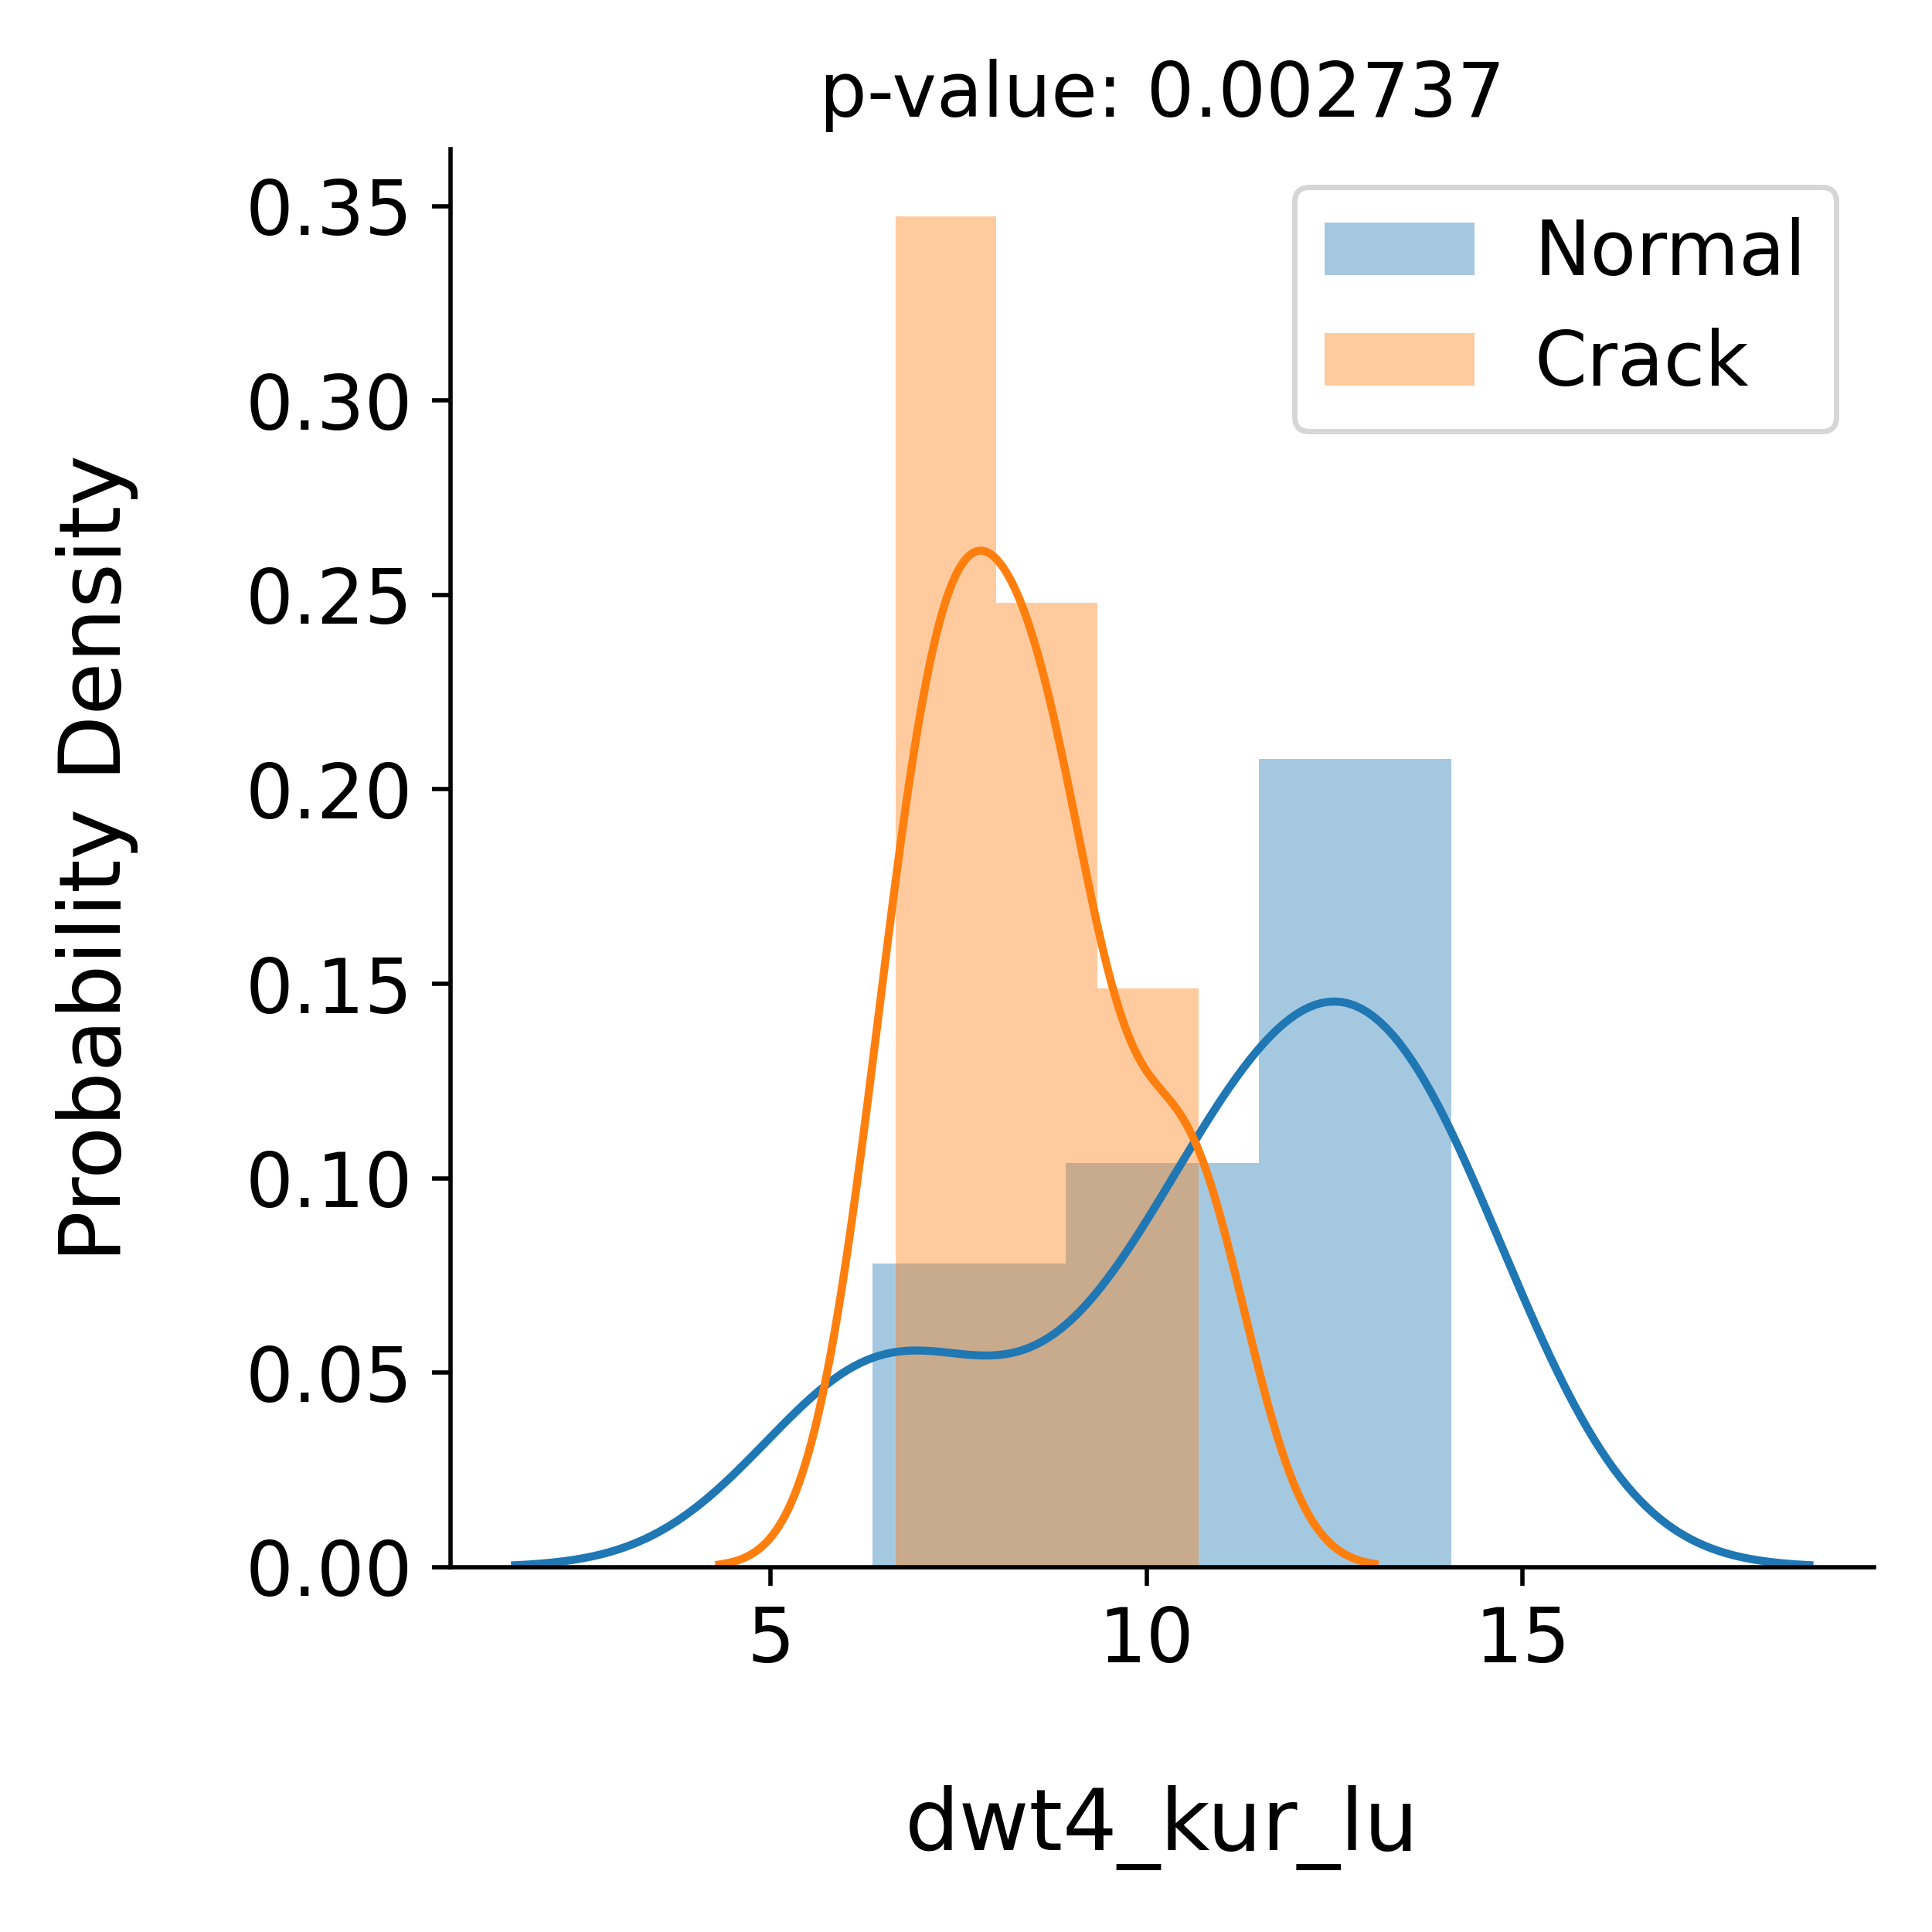
\includegraphics[width=0.8\textwidth]{fig/crack_detection_dwt4_kur_lu.png}
    \caption{Kurtosis of level 4 DWT coefficient of LU signal}
  \end{subfigure}
  \begin{subfigure}[t]{0.49\linewidth}
    \centering
    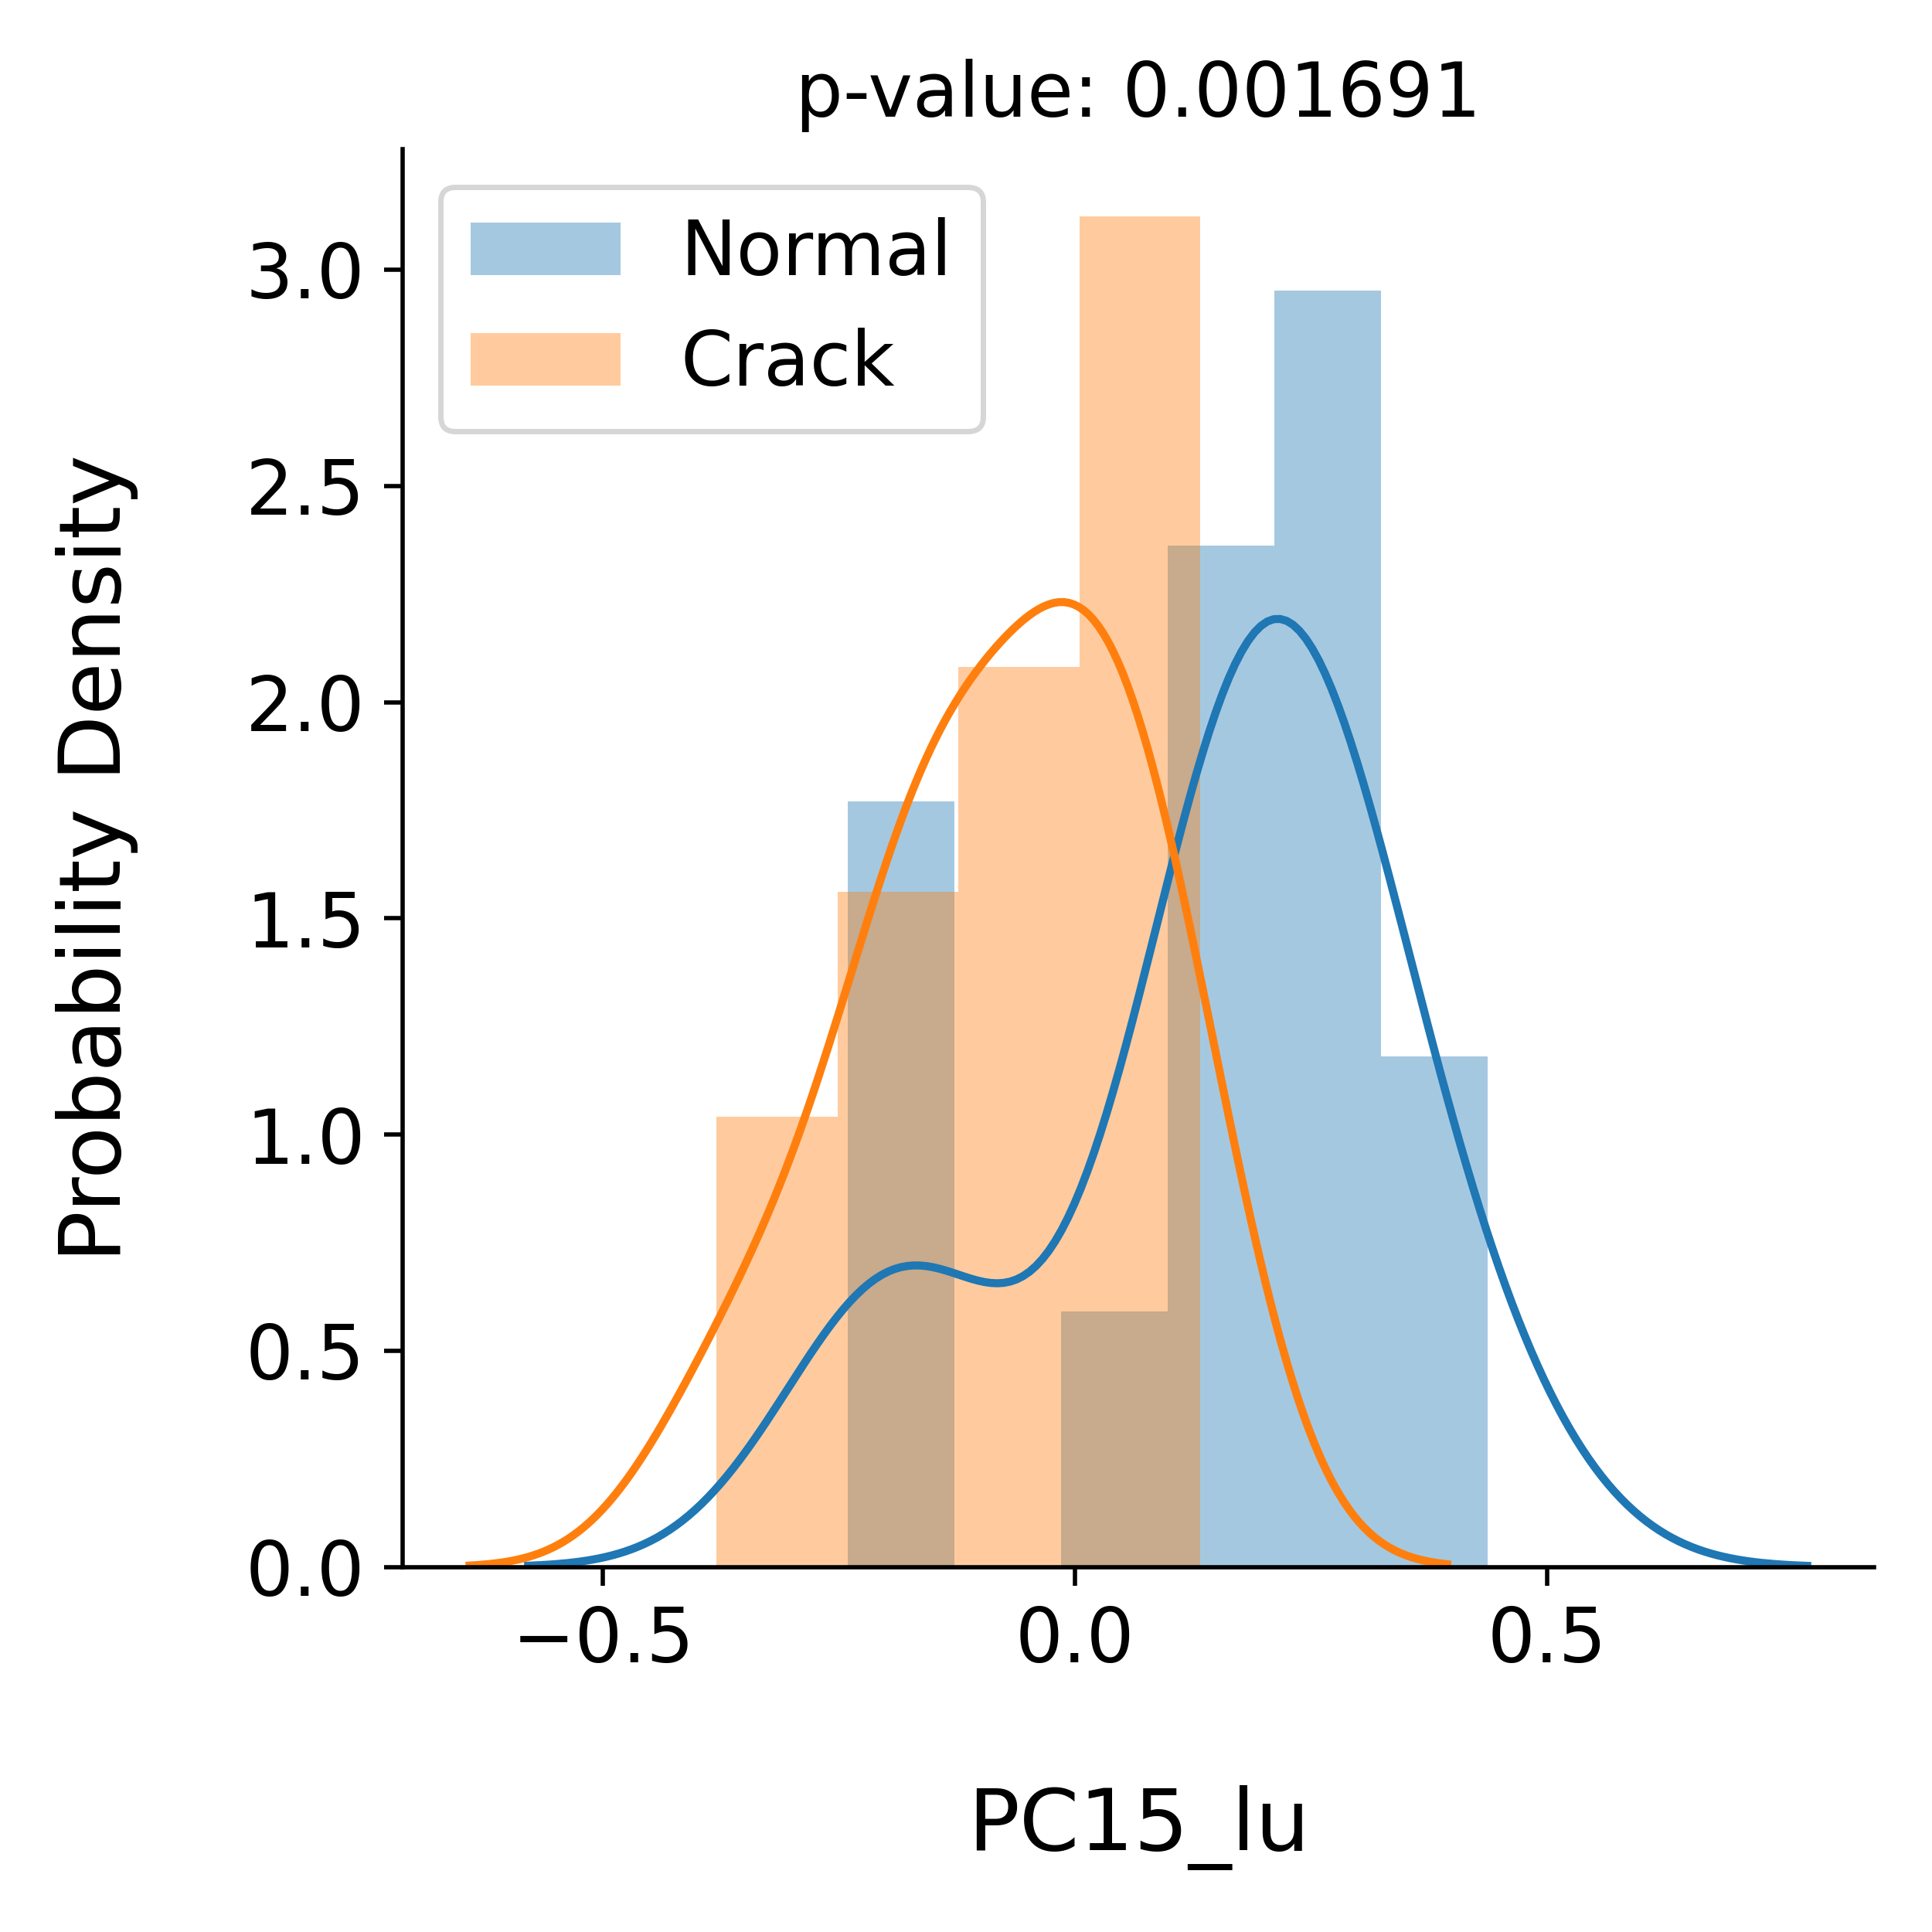
\includegraphics[width=0.8\textwidth]{fig/crack_detection_PC15_lu.png}
    \caption{Principal component 15 of LU signal}
  \end{subfigure}
  \begin{subfigure}[t]{0.49\linewidth}
    \centering
    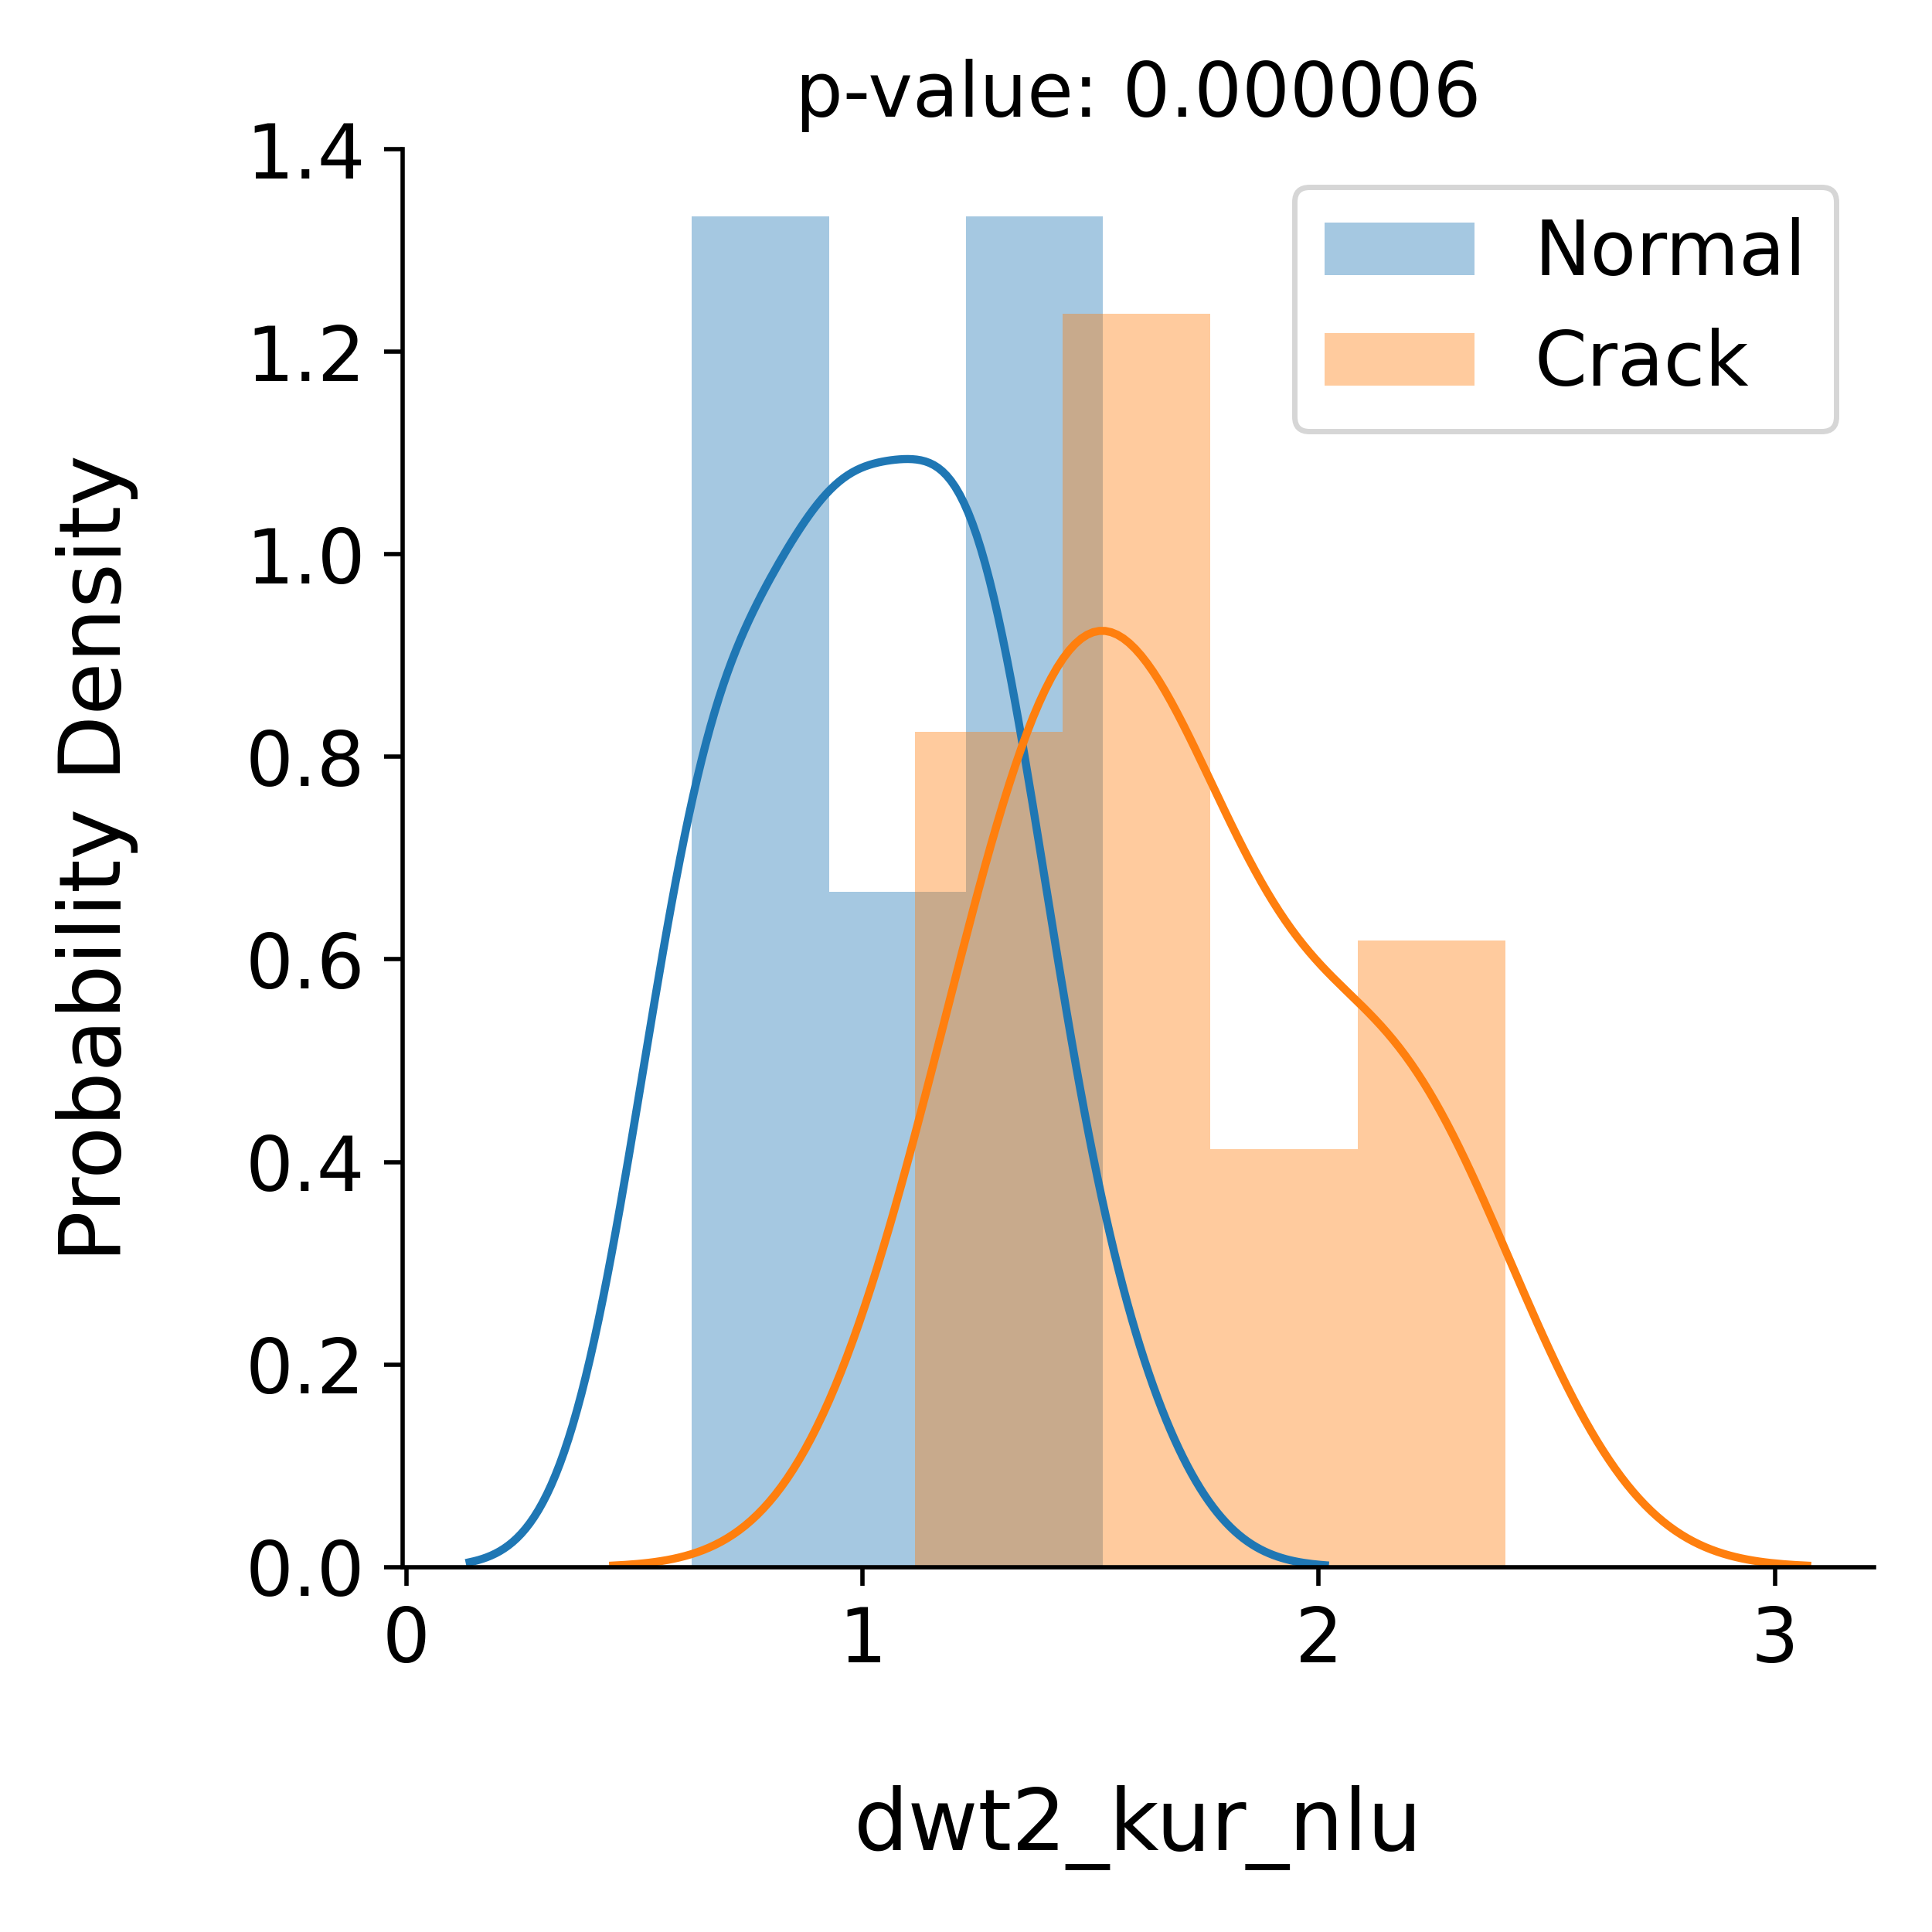
\includegraphics[width=0.8\textwidth]{fig/crack_detection_dwt2_kur_nlu.png}
    \caption{Kurtosis of level 2 DWT coefficient of NLU signal}
  \end{subfigure}
  \begin{subfigure}[t]{0.49\linewidth}
    \centering
    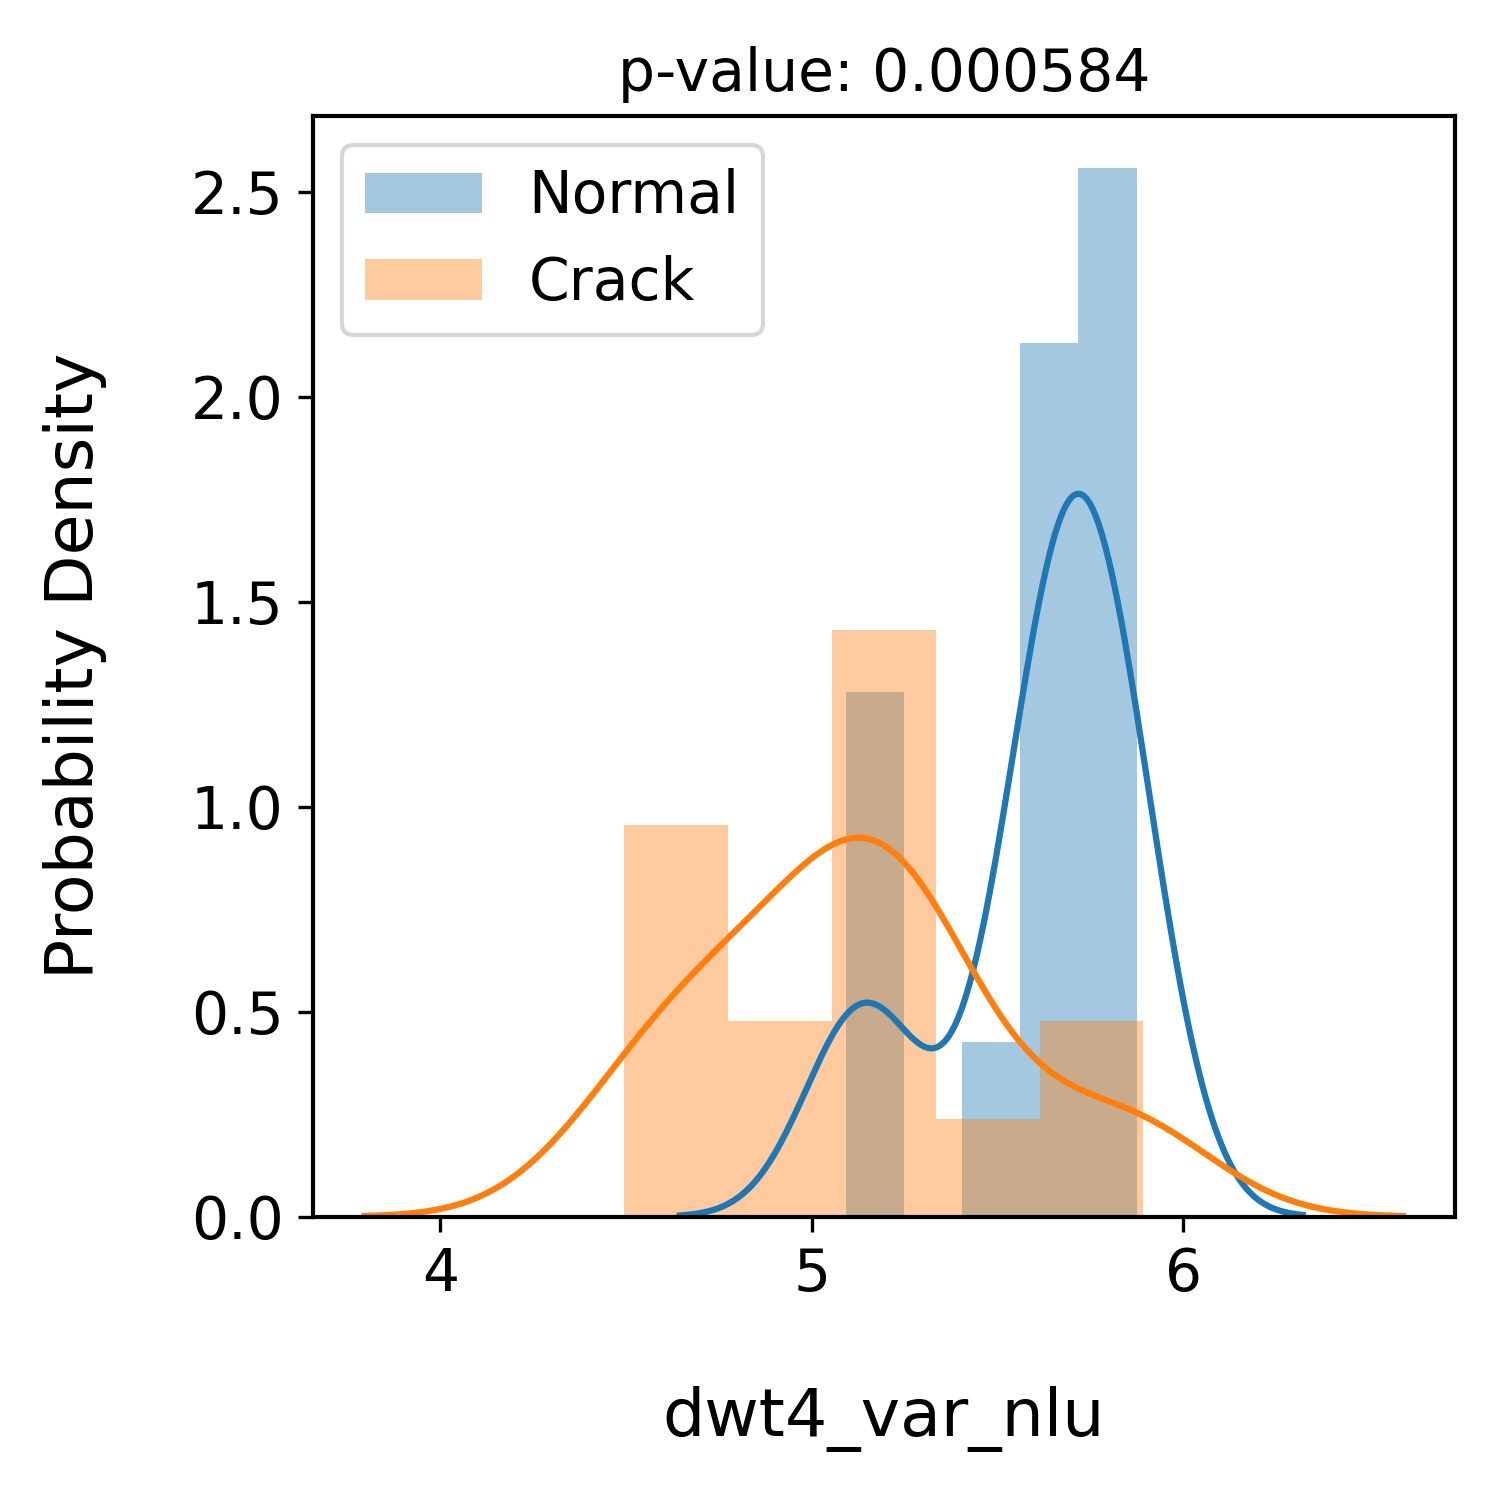
\includegraphics[width=0.8\textwidth]{fig/crack_detection_dwt4_var_nlu.png}
    \caption{Variance of level 4 DWT coefficient of NLU signal}
  \end{subfigure}
  \begin{subfigure}[t]{0.49\linewidth}
    \centering
    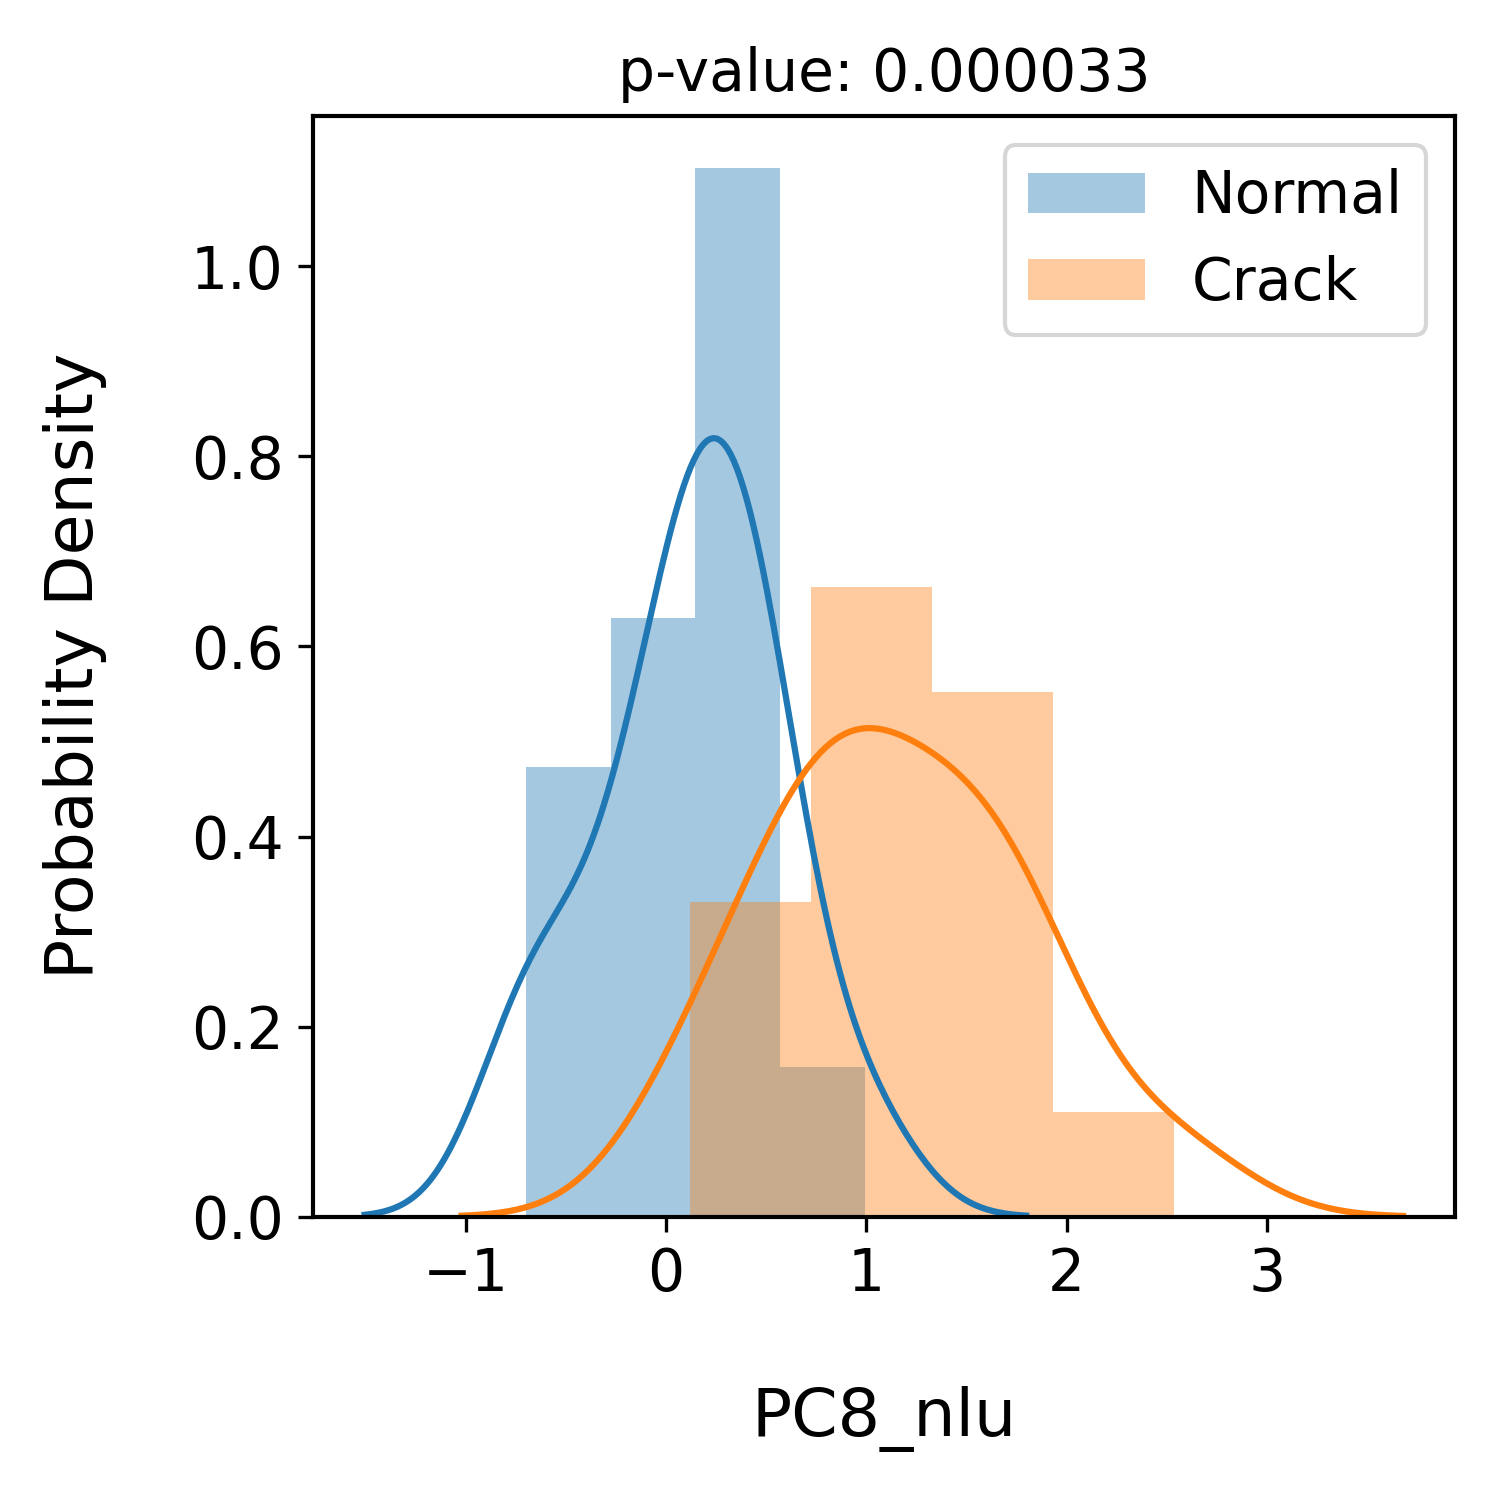
\includegraphics[width=0.8\textwidth]{fig/crack_detection_PC8_nlu.png}
    \caption{Principal component 8 of NLU signal}
  \end{subfigure}

  \caption{Probability density plots for selected LU and NLU features}
  \label{fig: crack detection feat dist}
\end{figure} % for REGGRESSION in "reg.tex"
\chapter{Conclusion} % for CONCLUSION in "concl.tex"


%%%%%%%%%%%%%%%%%%%%%%%%%%%%%%%%%%%%%%%%%%%%%%%%%%%%%%%%%%%%%%%%%%%%%%%%%%%%%%%
% APPENDIX
%
\appendix
%\include{apx}

\backmatter

%%%%%%%%%%%%%%%%%%%%%%%%%%%%%%%%%%%%%%%%%%%%%%%%%%%%%%%%%%%%%%%%%%%%%%%%%%%%%%%
% BIBLIOGRAPHY
%
\bibliographystyle{IEEE_ECE}
% Put references in BibTeX format in thesisrefs.bib.
\bibliography{thesisrefs}


%%%%%%%%%%%%%%%%%%%%%%%%%%%%%%%%%%%%%%%%%%%%%%%%%%%%%%%%%%%%%%%%%%%%%%%%%%%%%%%
% AUTHOR'S BIOGRAPHY
% As of 10/03/2011, Author's Biography or Vita no longer accepted by Grad College

\end{document}
\endinput
